
\documentclass[georeport,12pt]{geophysics}

\usepackage{amsmath}
\usepackage{amssymb}
\usepackage{amsthm}
\usepackage{amscd}
\usepackage{setspace}
\usepackage{wasysym}
\usepackage{algorithm}
\usepackage{algpseudocode}


\newcommand{\mb}{\mathbf}
\newcommand{\ba}{\mathbf{a}}
\newcommand{\bx}{\mathbf{x}}
\newcommand{\bxi}{\mathbf{\xi}}
\newcommand{\bk}{\mathbf{k}}
\newcommand{\bv}{\mathbf{v}}
\newcommand{\bff}{\mathbf{f}}
\newcommand{\bu}{\mathbf{u}}
\newcommand{\by}{\mathbf{y}}
\newcommand{\bz}{\mathbf{z}}
\newcommand{\bh}{\mathbf{h}}
\newcommand{\bR}{\mathbf{R}}

\newtheorem{lemma}{Lemma}
\newtheorem{theorem}{Theorem}
\newtheorem{alg}{Algorithm}
\newtheorem{remark}{Remark}
\newtheorem{cor}{Corollary}
\newtheorem{example}{Example}
\newtheorem{definition}{Defenition}



\setfigdir{.}

\begin{document}
\title{Efficient Computation of Extended Surface Sources}
\author{William W. Symes\\
 %\thanks{The Rice Inversion Project,
  Department of Computational and Applied Mathematics,\\
  Rice University,Houston TX 77251-1892 USA,\\
  email {\tt symes@rice.edu},\\
ORCID 0000-0001-6213-4272}

\lefthead{Symes}

\righthead{Approximate Source Inversion}

\maketitle
\begin{abstract}
Source extension is a reformulation of inverse problems in wave propagation, that at least in some cases leads to computationally tractable iterative solution methods. The core subproblem in all source extension methods is the solution of a linear inverse problem for a source (right hand side in a system of wave equations) through minimization of data error in the least squares sense with soft imposition of physical constraints on the source via an additive quadratic penalty. A variant of the time reversal method from photoacoustic tomography provides an approximate solution that can be used to precondition Krylov space iteration for rapid convergence to the solution of this subproblem. An acoustic 2D example for sources supported on a surface, with a soft contraint enforcing point support, illustrates the effectiveness of this preconditioner.
\end{abstract}

\noindent {\bf Keywords:} inverse problems, wave propagation, time
reversal, Krylov subspace methods, preconditioning

% \inputdir{../sseprecond/project}
\inputdir{.}

\section{Introduction}
Full Waveform Inversion (FWI) can be described in terms of 
\begin{enumerate}
\item a linear wave operator $L[{\bf c}]$, depending on a vector of
  space-dependent coefficients ${\bf c}$ and acting on causal vector wavefields $\bu$ vanishing in negative time:
\begin{equation}
\label{eqn:init}
\bu \equiv 0, t \ll 0; 
\end{equation}
\item a trace sampling operator $P$ acting on wavefields and producing data traces;
\item and a (vector) source function (of space and time) $\bff$ representing energy input to the system. 
\end{enumerate}
The basic FWI problem is: given data $d$, find ${\bf c}$ so that data
is fit and wave physics are honored, that is, 
\begin{equation}
\label{eqn:fwi}
P\bu \approx d \mbox{ and } L[\bf{c}]\bu = \bff.
\end{equation}
The source function $\bff$ may be given, or to be determined along
with $\bf{c}$.
%The energy source $\bff$ may also be largely undetermined, apart from some known characteristics such as localization in space and/or time. In fact, additional source degrees of freedom, beyond those needed to describe physically realized sources, may be useful in rendering the FWI problem \ref{eqn:fwi} more amenable to numerical solution, via so-called extended modeling (see \cite{geoprosp:2008}, \cite{LeeuwenHerrmannWRI:13}, \cite{HuangNammourSymesDollizal:SEG19}, and many references cited there). Therefore it is natural to view $\bff$ as also an unknown in formulating the problem \ref{eqn:fwi} via nonlinear least squares:
The task \ref{eqn:fwi} may be cast as a nonlinear least squares problem: 
\begin{equation}
\label{eqn:ols}
\mbox{choose } {\bf c} \mbox{ to minimize } \|PL[{\bf c}]^{-1}\bff -d \|^2.
\end{equation}
Practical variants of the least squares problem \ref{eqn:ols}
typically augment the objective with additive penalties or other
constraints \cite[]{VirieuxOperto:09,Fichtner:10,Schuster:17}. 

As is well-known, local optimization methods are the only feasible
approach given the dimensions of a typical instance of \ref{eqn:fwi},
and those have a tendency to stall at uninformative model estimates
due to ``cycle-skipping''. This phenomenon is often interpreted as the
capture of optimizing sequences at local minima of the nonlinear objective
function in \ref{eqn:ols} far from the global minimum, or at least not
possessing the characteristics of a useful solution. See for
example \cite{GauTarVir:86,VirieuxOperto:09,PladysBrossierLiMetivier:GEO21}.

Source extension is one approach to avoiding this``cycle-skipping''
obstacle. It consists in imposing the wave equation as a soft
constraint, allowing the source field $\bff$ to have more degrees of
freedom than is permitted by a faithful model model of the seismic
experiment, and constraining these additional degrees of freedom by
means of an additive quadratic penalty modifying the problem
\ref{eqn:ols}:
\begin{equation}
\label{eqn:esi}
\mbox{choose } {\bf c}, \bff \mbox{ to minimize } \|PL[{\bf c}]^{-1}\bff -d \|^2 + \alpha^2 \|A\bff\|^2 
\end{equation}
The linear operator $A$ penalizes deviation from known (or assumed)
characteristics of the source function - its null space consists of
feasible (or ``physical'') source models.
\cite{HuangNammourSymesDollizal:SEG19} present an overview of the
literature on source extension methods, describing a variety of
methods to add degrees of freedom to physical source model.

The present paper concerns {\em surface source extension}: physical
sources are presumed to be concentrated spatially at points $\bx_s$
in space, whereas their extended counterparts are permitted to spread
energy over a {\em source surface} containing the physical source spatial
locations. Similarly, the receiver spatial locations are confined to a
{\em receiver surface}. A simple choice for the penalty operator $A$ is then
multiplication by the distance $|\bx-\bx_s|$ to the physical source
location:
\begin{equation}
  \label{eqn:penop}
  (A\bff)(\bx,t) = |\bx-\bx_s|\bff(\bx,t)
\end{equation}
I shall use this choice of penalty operator whenever a specific choice
is necessary in the development of the theory below.

This paper presents a numerically efficient approach to solving the
{\em source subproblem} of problem \ref{eqn:esi}:
\begin{equation}
\label{eqn:esis}
\mbox{given } {\bf c}, \mbox{ choose } \bff \mbox{ to minimize }
\|PL[{\bf c}]^{-1}\bff -d \|^2 + \alpha \|A\bff\|^2 
\end{equation}
Solution of this subproblem is an essential component of {\em variable
  projection} algorithms for solution of the nonlinear inverse problem
\ref{eqn:esi}. Variable projection is not merely a convenient choice
of algorithm for this purpose: it is in some sense essential, see for
example \cite{Symes:SEG20}. It replaces the nonlinear
least squares problem \ref{eqn:esi} with a {\em reduced} problem, to
be solved iteratively. Each iteration involves solution of the
subproblem \ref{eqn:esis}. Therefore efficient solution of the
subproblem is essential to efficient solution of the nonlinear problem
via variable projection.

The modeling operator $PL[{\bf c}]^{-1}$ and the penalty operator $A$ defined in \ref{eqn:penop} are linear, so the source
subproblem is a linear least squares problem. Under some additional
assumptions to be described below, I shall show how to construct an
accurate approximate solution operator for problem
\ref{eqn:esis}. This approximate solution operator may be used to
accelerate (``precondition'') Krylov space methods for the solution of the surface source
subproblem \ref{eqn:esis}. I will fully describe a preconditioner for a special
case of the source subproblem \ref{eqn:esis}, in which ${\bf u}$ is an
acoustic field, $L[{\bf c}]$ is the wave operator of linear
acoustodynamics, and the source and receiver surfaces are horizontal
planes. Numerical examples in this setting suggest the
effectiveness of this acceleration.

I will use two 2D numerical models 
throughout to illustrate the theory. In both, horizontal lines serve as
source and receiver surfaces. The first is a ``crosswell'' or slab
configuration with an acoustic lens positioned between a deeps source
and a shallower line of 
receivers, resulting in markedly triplicated arrivals. The goal in
this first example is to construct a surface source that explains the data in a
homogeneous medium (that is, inversion in a wrong velocity, emulating
the early iterations of FWI based on extended modeling). The second is a layered
model in which velocity increases with depth, resulting the formation
of diving waves. This configuration simulates an
ocean-bottom node and a line of near-surface sources: the roles of
source and receiver are switched for computational convenience. In
this second example, the diving wave arrivals are isolated (by an
appropriate mute operator) and a
source constructed that explains them alone.

The next section defines the modeling operator $PL[{\bf c}]$, its
adjoint, and important specializations (pressure vs. normal velocity
sources and data). It also introduces the two 2D examples mentioned
above.  The following section constructs an approximate inverse of the
modeling operator by time reversal (as suggested by work in
photoacoustic tomography), and illustrates its efficacy in the two
examples. This construction requires extraction of
velocity data, or equivalently a surface source, from pressure data.
The subsequent sections describe this pressure-to-source operator,
express the approximate inverse as the modeling operator adjoint in
weighted norms (thus establishing that the modeling operator is {\em
  approximately unitary} in the sense of these norms), explain how to
use this construction to precondition Conjugate Gradient iteration,
and organize the preconditioning computation so as to involve only one
extra and relatively inexpensive wave propagation calculation. I use
the 2D examples to illustrate each of
these developments. The paper ends with a brief
discussion-and-conclusion section, reviewing what has been
accomplished and listing a few of the many questions left open.

%I will fully describe a preconditioner for a special
%case of the source subproblem \ref{eqn:esis}, in which ${\bf u}$ is an
%acoustic field, $L[{\bf c}]$ is the wave operator of linear
%acoustodynamics, and the source and receiver surfaces are horizontal
%planes.
%spatial positions of traces extracted by $P$ lie
%on a depth plane $z=z_r$, and the positions at which the extended
%source $\bff$ is nonzero lie on another, parallel, depth plane $z=z_s$. 
%That is, sources take the form of a combination of constitutive law
%defect and normal force,
%\begin{equation}
%  \label{eqn:surfsrc}
%  \bff(x,y,z,t) = h_s(x,y,t)\delta(z-z_s)(1,0,0,0)^T + f_s(x,y,z,t)(0,0,0,1)^T
%\end{equation}
%and the sampling operator $P$ is defined by
%\begin{equation}
%  \label{eqn:surfsam}
%  P\bu(x,y,t) =
%\end{equation}
%supported on $z=z_s$, and similar
%surface vertical loads.
%This configuration simplifies the presentation of the
%approximate solution construction.

\section{Overview}

The preconditioner construction is closely related to the time
reversal method in photoacoustic tomography
\cite[]{StefanovUhlmannIP:09,Hristova:09}. A simplified mathematical
translation of this medical imaging task is to infer the initial
excess pressure distribution over a fluid-containing region at time
$t=0$ from measurements of the pressure on a surface enclosing the
fluid over a time interval $0 \le t \le t_{\rm max}$. This problem
clearly has strong similarities to, but also differences from, the
problem studied here. The time reversal method presumes that the
pressure field has returned to equilibrium (zero excess pressure), or close to it, at the
final time $t=t_{\rm max}$ Then the field can be (at least
approximately) viewed as the backwards-in-time initial boundary value
problem with zero final conditions at $t=t_{\rm max}$, and boundary
values given by the measurements. Evolving the field backwards in time
backwards to $t=0$ thus solves the problem. Except in special
circumstances, the pressure field never actually vanishes at finite
time, so the solution is approximate.

The seismic surface source extension proplem \ref{eqn:esis} differs in
several obvious ways from the photoacoustic setting. The measurement
or receiver surface does not surround the region of wave
propagation. It is not the initial pressure time-slice at $t=0$ that
is to be determined, but a time-extended source $\bff$ confined to a
surface. The penalty operator has no analogue in the basic
photoacoustic problem description. Finally, once these obstacles are
overcome, using the approximate solution operator to accelerate Krylov
iteration for solution of the optimization problem \ref{eqn:esis}
requires that the operator be identified as the adjoint of the
modeling operator with respect to suitable inner products in its domain
and range. In the pages to follow, I will address each of these issues.

First, reverse-time propagation can be localized via ray theory,
within high-frequency asymptotic approximation. This step requires
some assumptions about the ray fields: all rays responsible for significant
energy in the receiver data must arrive from the source surface, and must cross the source and receiver
surfaces transversally, that is, making non-zero angles. Also, the
rays must approach source and receiver surfaces from one side or the
other (``the inside''), so that locally the surfaces can be treated as boundaries of
propagation domains. With these assumptions, reverse-time propagation
of the receiver data
closely approximates the acoustic fields near the source surface. Next
observe that for a causal field with a surface pressure source (with a
continuous pressure field across the surface), the source is
proportional to the jump in the (particle) velocity field. Moreover,
to leading order in frequency, the velocity field switches sign at the
surface, so the jump is just twice the sampled value on the
surface. Thus reverse-time propagation and reading off the velocity
field on the source surface yields
a source that reproduces the pressure data, within an asymptotically small error.
%Preconditioning amounts to a change of
%norm in the domain and range spaces of the modeling operator. In this
%case, the modfied norms are weighted $L^2$, and the weight operators
%map pressure to corresponding surface source on the source and
%receiver planes.

This is the essence of the approximate solution of the problem
\ref{eqn:esis} for penalty weight $\alpha=0$. To see how Krylov
iteration might be accelerated, note that time-reverse propagation of
the receiver pressure values may be represented by a time-reverse
source propagation, with the source constructed from the velocity
field at the receiver surface. Moreover, the reverse-time
source-to-pressure propagation is the transpose (adjoint) of the
forward-time source-to-pressure propagation - this is a very simple
version of the adjoint state construction \cite[]{Plessix:06}. So the
approximate inverse is: conversion of pressure to source at the
receiver surface, followed by the adjoint of the modeling operator,
followed by the conversion of pressure to source at the source
surface. This sequence precisely describes the adjoint of the modeling
operator with respect to weighted norms in the spaces of source and
receiver data, with the weight operators being the
pressure-to-source operators. That this construction results in an
approximate inverse means that the modeling operator is approximately
unitary with respect to these weighted norms, which in turn implies
that the preconditioned conjugate gradient algorithm should converge rapidly.

This pressure-to-source map is closely related to the ``hyperbolic
Dirichlet-to-Neumann'' operator that plays a prominent role in
photoacoustic tomography and other wave inverse problems
\cite[]{Rachele:00,StefUhl:05}. \cite{HouSymes:EAGE16} demonstrated a
very similar preconditioner for Least Squares Migration, also for its
subsurface offset extension \cite[]{HouSymes:16}, motivated by
\cite{tenKroode:12}. These constructions also involve the
Dirichlet-to-Neumann operator. This concept also turns up in hidden
form in the work of Yu Zhang and collaborators on true amplitude
migration
\cite[]{YuZhang:14,TangXuZhang:13,XuWang:2012,XuZhangTang:11,Zhang:SEG09}.

FInally, the $\alpha=0$ case is not sufficient: the penalty operator
$A$ is an essential component of the nonlinear inverse propblem
\ref{eqn:esi}. As it turns out, $A$ commutes with the other operators
involved - approximately, but that is enough. Therefore the effect of
$A$ can be compensated with an easily-computed factor, whence the
preconditioned acceleration extended to the case $\alpha > 0$. 

%The obvious computation of the pressure-to-source map - prescribe the
%pressure, solve the wave equation with this boundary condition, read
%off the equivalent source - suffers from intrinsic numerical
%inaccuracy. I suggest an alternative computationally feasible
%approach, via economical short-distance wave propagation. Since the
%map is symmetric only in an approximate, asymptotic sense, it must be
%symmetrized for use as a Krylov preconditioner. I describe a
%symmetrization procedure that requires no further wave computations
%beyond those necessary to compute the action of the operator itself.


The discussion in this paper is formal and incomplete, in the sense
that some important mathematical underpinnings are only
sketched. I will treat the modeling operator $PL[{\bf c}]^{-1}$ as if
it mapped square integrable surface sources to square integrable sampled
data. This is not true in full generality: while the surface source
problem has distribution solutions, they are not generally square
integrable (finite acoustic field energy). Even if the solutions have
finite energy, they do not in general have well-defined
restrictions to lower-dimensional sets. In other words, the action of
the sampling
operator $P$ on the receiver surface is not well-defined for arbitrary
finite-energy acoustic fields. Thus the modeling operator envisioned above
is not be well-defined, strictly speaking.

This phenomenon is related to the ill-posedness of wave equations as
evolution equations in spatial variables, an observation attributed to
Hadamard (see \cite{CourHil:62}, Chapter 6, section 17). A number of
authors have described precise forms of the ray conditions described
above, and shown how these conditions lead to the desired behaviour of
the modeling operator, that is, mapping of finite energy sources to
finite energy data, or equivalent properties
\cite{Payn:75,Symes:83,Lasi:86,LasLionsTrig:86,Lasi:87, BaoSy:91b}.
Elaboration of these mathematical details is beyond the scope of this
paper, which aims instead to explore the algorithmic consequences of
the mathematical structure implied by the nongrazing hypothesis.

%Some
%constraint on the acoustic field, beyond finite energy, is mandatory
%in any precise mathematical formulation the inverse problems
%\ref{eqn:esi} and \ref{eqn:esis}. I assume throughout that that
%high-frequency energy contributing to the measured data
%(output of the modeling operator) travels {\em only} along rays crossing the source
%and receiver surfaces transversally, that is, making non-zero angles
%with the tangent planes. I will call sources, sampled data, and
%acoustic fields with this property {\em non-grazing}. Note that the
%non-grazing property restricts the behaviour of acoustic fields near the
%source and receiver surfaces - what the fields do elsewhere is their
%own business.

%A further restriction turns out to be necessary: {\em all} of the rays
%associated with significan energy in the data must originate on
%the source surface and have the {\em incoming} property (essentially
%what is known in seismology as {\em downgoing}). This assumption uses
%an orientation of the source surface to distinguish inward and outward
%directions, and mandates that the rays in question all cross the
%source surface and propagate inwards in forward time. By symmetry,
%rays arriving at the receiver surface should propagate outward, with
%proper choice of orientation. These assumptions are also local at the
%source and receiver surfaces, and are often a natural consequence of
%the acquisition and ray geometry, as is the case in the two examples
%mentioned above.




\section{Operators}

For acoustic wave physics, the coefficient vector is
$\bf{c}=(\kappa,\rho)^T$, with components bulk modulus $\kappa$ and
density $\rho$, and the state vector $\bu=(p,\bv)^T$ consists of
pressure $p$ (a scalar space-time field) and particle velocity $\bv$
(a vector space-time field). The wave operator $L[\bf{c}]$ is:
\begin{equation}
\label{eqn:aweop}
L[\bf{c}]\bf{u} = 
\left(
\begin{array}{c}
\frac{1}{\kappa}\frac{\partial p}{\partial t}  + \nabla \cdot \bv, \\
\rho\frac{\partial \bv}{\partial t} + \nabla p.
\end{array}
\right) 
\end{equation}
That is,
\begin{equation}
  \label{eqn:awemat}
  L[{\bf c}] = \left(
    \begin{array}{cc}
      \frac{1}{\kappa}\frac{\partial}{\partial t} & \nabla \cdot \\
      \nabla & \rho \frac{\partial}{\partial t}
    \end{array}
  \right)
\end{equation}
$L[{\bf c}]$ has a well-defined inverse in the sense of distributions
if it is restricted to either causal or anti-causal vector wavefields.

Since all of the operators in the discussion that follows depend on
the coefficient vector $\bf{c}$, I will suppress it from the notation,
for example, $L=L[\bf{c}]$.

Most of what follows is valid for any space dimension $n >0$. I will
describe the theory for $n=3$, write $\bx=(x,y,z)^T$ for the spatial
coordinate vector, and refer to the third (vertical) coordinate of
particle velocity $\bv$ as $v_z$. For computational convenience, the
examples are two-dimensional.

The surface source extension replaces point sources on or near a
surface in $\bR^3$ with source functions confined to the 
surface. The simplest example of this extended geometry specifies a
plane $\{(x,y,z,t): z=z_s\}$ at source depth $z_s$ as the surface. For
acoustic modeling, surface sources are combinations of constitutive law
defects and loads normal to the surface, localized on $z=z_s$. That
is, right-hand sides in the system $L\bu=\bff$ take the form
$\bff(\bx,t) = (h_s(x,y,t)\delta(z-z_s),
f_s(x,y,t)\bf{e}_z\delta(z-z_s))^T$ for scalar defect $h_s$ and normal
force $f_s$ ($\bf{e}_z=(0,0,1)$). With the choice $L$ given in
\ref{eqn:awemat}, the causal/anti-causal wave system $L\bu^{\pm}=\bff$
takes the form
\begin{eqnarray}
\label{eqn:awepm}
\frac{1}{\kappa}\frac{\partial p^{\pm}}{\partial t} & = & - \nabla \cdot \bv^{\pm} +
h_s \delta(z-z_s), \nonumber \\
\rho\frac{\partial \bv^{\pm}}{\partial t} & = & - \nabla p^{\pm} +
                                                f_s{\bf e} \delta(z-z_s),\nonumber \\
p^{\pm} & =& 0 \mbox{ for } \pm t \ll 0,\nonumber\\ 
\bv^{\pm} & = & 0 \mbox{ for } \pm t \ll 0.
\end{eqnarray}

\noindent {\bf Remark:} In system \ref{eqn:awepm} and many similar
systems to follow, I will use the shorthand
\[
  p^+ = 0 \mbox{ for } t \ll 0 
\]
to mean that $p^+$ is {\em causal}, that is,
\[
  \mbox{For some } T \in \bR, p^+(\cdot,t) = 0 \mbox{ for all } t <
  T.
\]
Similarly,
\[
  p^- = 0 \mbox{ for } t \gg 0 
\]
signifies that $p^-$ is anti-causal.

Extended forward modeling consists in solving \ref{eqn:awepm} and
sampling the solution components at receiver locations. For
simplicity, throughout this paper I will assume that the receivers are
located on another spatial plane $\{(x,y,z,t): z=z_r\}$ at receiver
depth $z_r$. The constructions to follow involve interchange of the
roles of $z_s$ and $z_r$ (that is, locating sources on $z=z_r$ and
receivers at $z=z_s$), so both require sampling operators: $P_s,P_r$
are the sampling operators on $z=z_s$, $z=z_r$ respectively. In
practice, sampling necessarily occurs at a discrete array of points
(trace locations), and over a zone of finite extent. In this
theoretical discussion, I will neglect the finite sample rate, and
regard the data, for example $P_rp^+$, as continuously sampled. The
output samples are necessarily muted, that is, non-zero only over a space-time domain
of finite extent. This mute, and any tapering applied to the data
traces, are regarded as part of the sampling operators $P_s,P_r$.

The causal/anti-causal vector
modeling operators ${\cal S}^{\pm}_{z_s,z_r}$ are defined in terms of
the solutions $(p^{\pm},\bv^{\pm})$ of the systems \ref{eqn:awepm} by
\begin{equation}
  {\cal S}^{\pm}_{z_s,z_r}(h_s,f_s)^T  = (P_rp^{\pm},P_r v_z^{\pm})^T,
  \label{eqn:fwd}
\end{equation}
The subscript signifies that sources are located on $z=z_s$,
receivers on $z=z_r$. It is necessary to include this information in
the notation, as versions of ${\cal S}^{\pm}$ with sources and receivers in
several locations will be needed later in the discussion.

Denote by $\Pi_i, i=0,1$ the projection on the first,
respectively second, component of a vector in $\bR^2$. The 
forward modeling operator from pressure source to pressure trace is
\begin{equation}
  \label{eqn:sdef}
  S^{\pm}_{z_s,z_r} = \Pi_0 {\cal S}^{\pm}_{z_s,z_r} \Pi_0^T 
\end{equation}
and the forward modeling operator from velocity source (normal force)
to velocity trace is
\begin{equation}
  \label{eqn:vdef}
  V^{\pm}_{z_s,z_r} = \Pi_1 {\cal S}^{\pm}_{z_s,z_r} \Pi_1^T 
\end{equation}

With these conventions, we can write the version of the source
subproblem \ref{eqn:esis} studied in this paper as
\begin{equation}
  \label{eqn:esisp}
  \mbox{find }h_s\mbox{ to minimize }\|S^{+}_{z_s,z_r}h_s- d\|^2 +
  \alpha^2\|Ah_s\|^2.
\end{equation}

The two examples mentioned in the introduction illustrate the setting
just described. The first example (Figure \ref{fig:olensrays0}) embeds
an acoustic (low-velocity) lens between a source surface at $z_s=3000$
(orange horizontal line) 
m and a receiver surface at $z_r=1000$ m (yellow horizontal line).  The data to be used in this
example results from a point source at $z_s=3500, x_s=3500$ m (orange
star). I have overlain the rays connecting this source point with the
data portion of the receiver surface: evidently all of the rays
involved cross the source and receiver surfaces transversally. Also,
regarding ``inwards'' as being ``upwards'' at the source surface,
``downwards'' at the receiver surface, it is clear that the data is
incoming at the source surface, outgoing at the receiver
surface.

\begin{figure}
  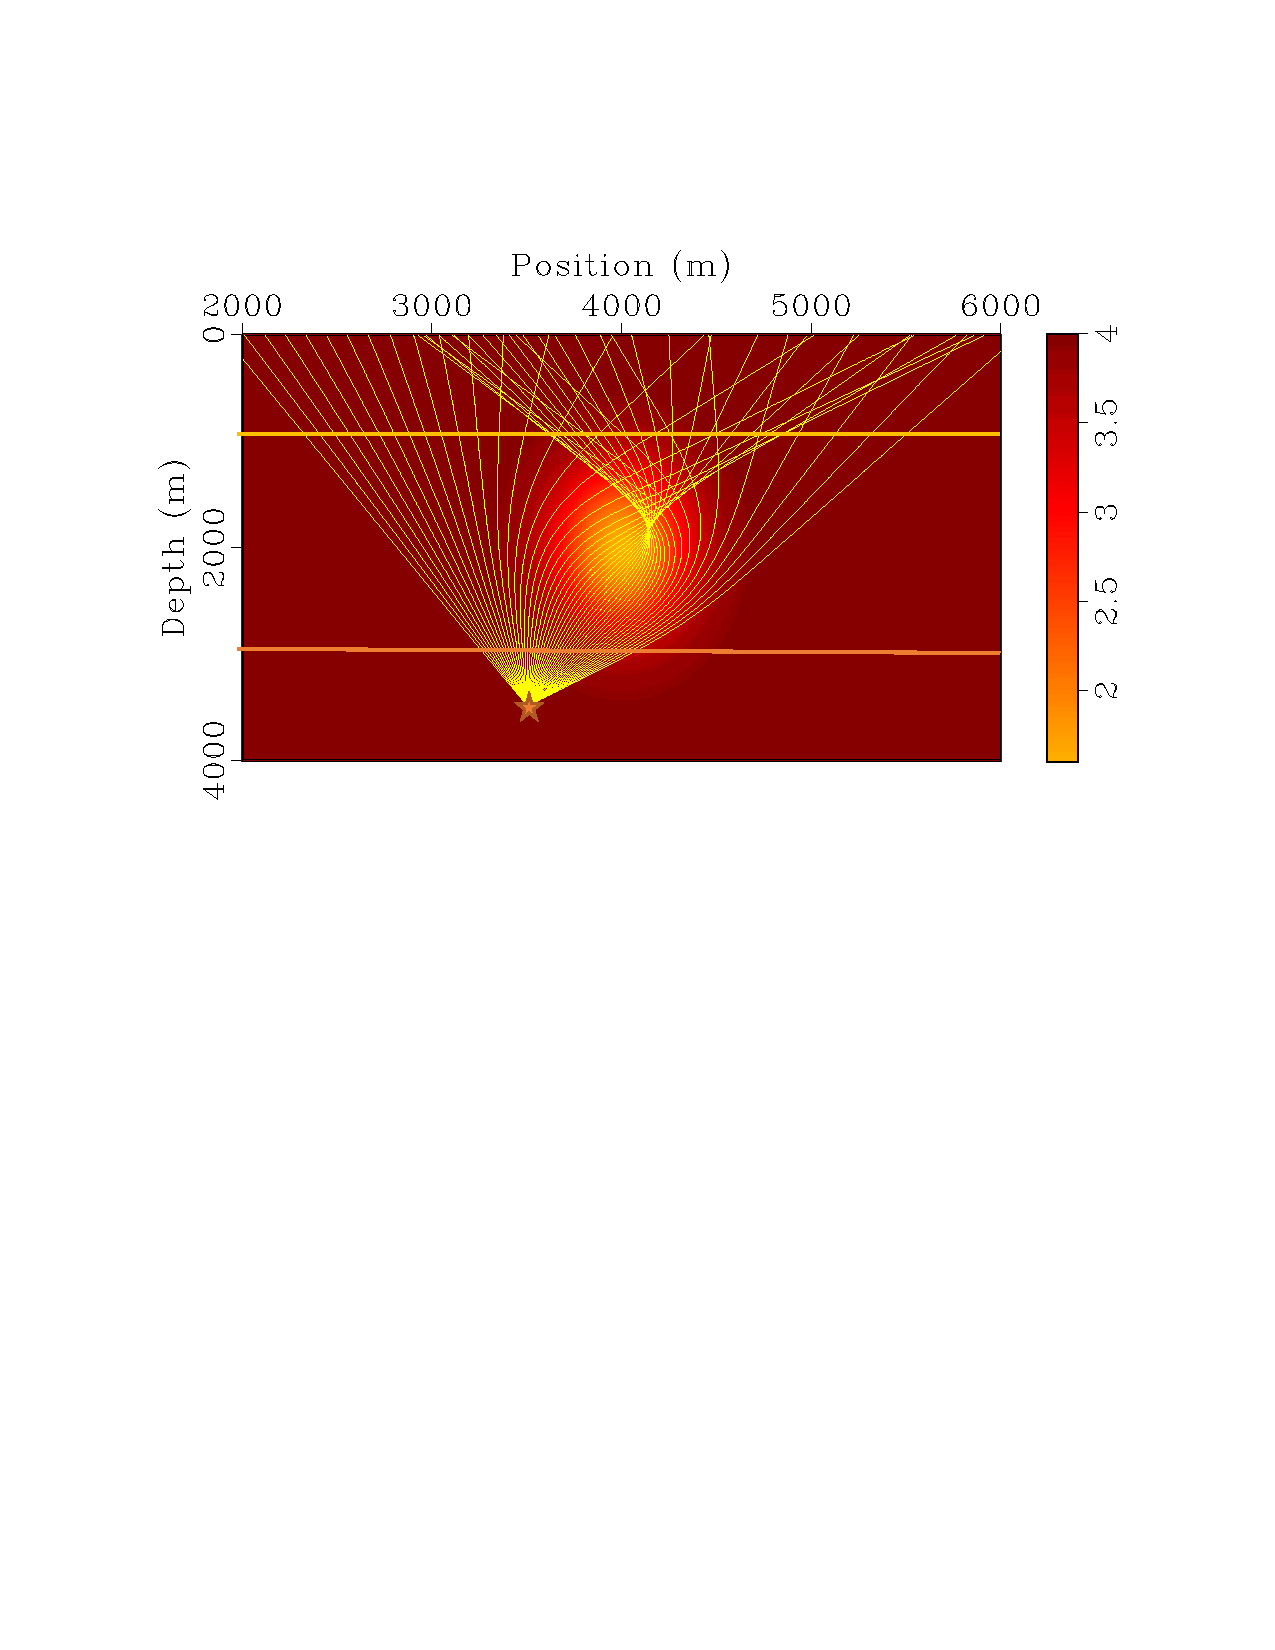
\includegraphics[width=\textwidth]{olensrays0.pdf}
  \caption{Bulk modulus with acoustic lens. Color scale unit is
    GPa. Orange horizontal line is source surface at depth $z_s= 3000$
    m, yellow horizontal
    line is receiver surface at depth $z_r=1000$ m. Point source location for data
    generation at $(3500, 3500)$ m indicated with star. Overlain with rays from point
    source to receiver surface.}
  \label{fig:olensrays0}
\end{figure}

%\ref{fig:drecplh0}, \ref{fig:dfwdplh0}
Figure \ref{fig:drecplh0} shows the gather $P_rp_{\rm pt}^{+}$, where
$p_{\rm pt}^{+}$ is causal field generated by the point source at
$(3500,3500)$ m with a trapezoidal bandpass filter wavelet having
significant energy between 1 and 12.5 Hz. The mute embedded in $P_r$
limits trace positions to 2000 m $ \le x_r \le $ 6000 m, and times to
1.2 s $ \le t \le $ 3 s.

Figure \ref{fig:dsrcphh0} displays an extended (pressure) source $h_s$, in the form of
traces in the spatial range 2000 m $ \le x_r \le $ 6000 m and time
range 0 s $\le t \le $ 2 s. The modeling operator output $S_{z_s,z_r}^+h_s$,
obtained from the causal solution $(p^+, \bv^+)$ of \ref{eqn:awepm}
with this choice of $h_s$ and $f_s=0,$ by application of the sampling
operator $P_r$ to $p^+$, are shown in Figure \ref{fig:dfwdplh0}.

\noindent {\bf Remark:} The close resemblance between Figures
\ref{fig:drecplh0} and \ref{fig:dfwdplh0} is not accidental  - the
extended source $h_ s$ shown in Figure \ref{fig:dsrcphh0} is constructed
so that $S^++_{z_s,z_r}h_s$ (Figure \ref{fig:dfwdplh0}) closely
approximates the point source gather $P_r p^+_{\rm pt}$ (Figure
\ref{fig:drecplh0}). This construction will be explained in the next section.

\begin{figure}
  \centering
  \subfloat[\label{fig:drecplh0}]{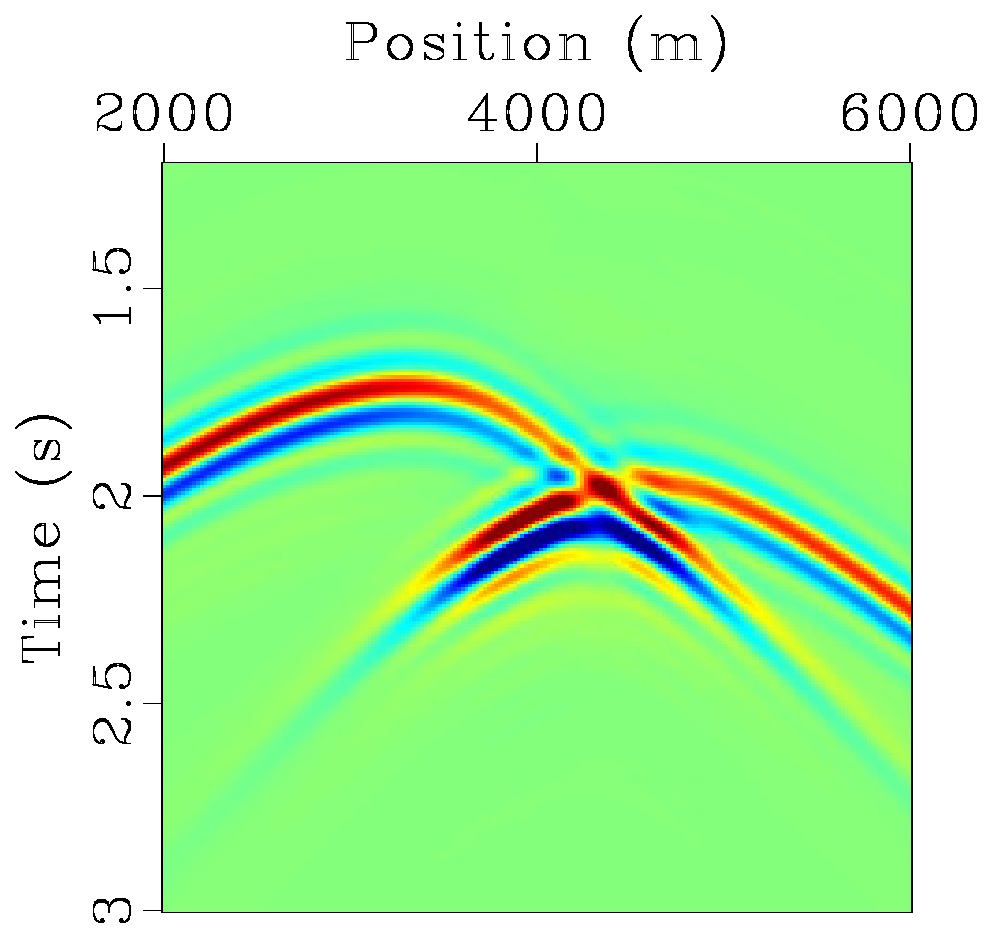
\includegraphics[width=0.32\textwidth]{drecplh0.pdf}}
  \subfloat[\label{fig:dsrcphh0}]{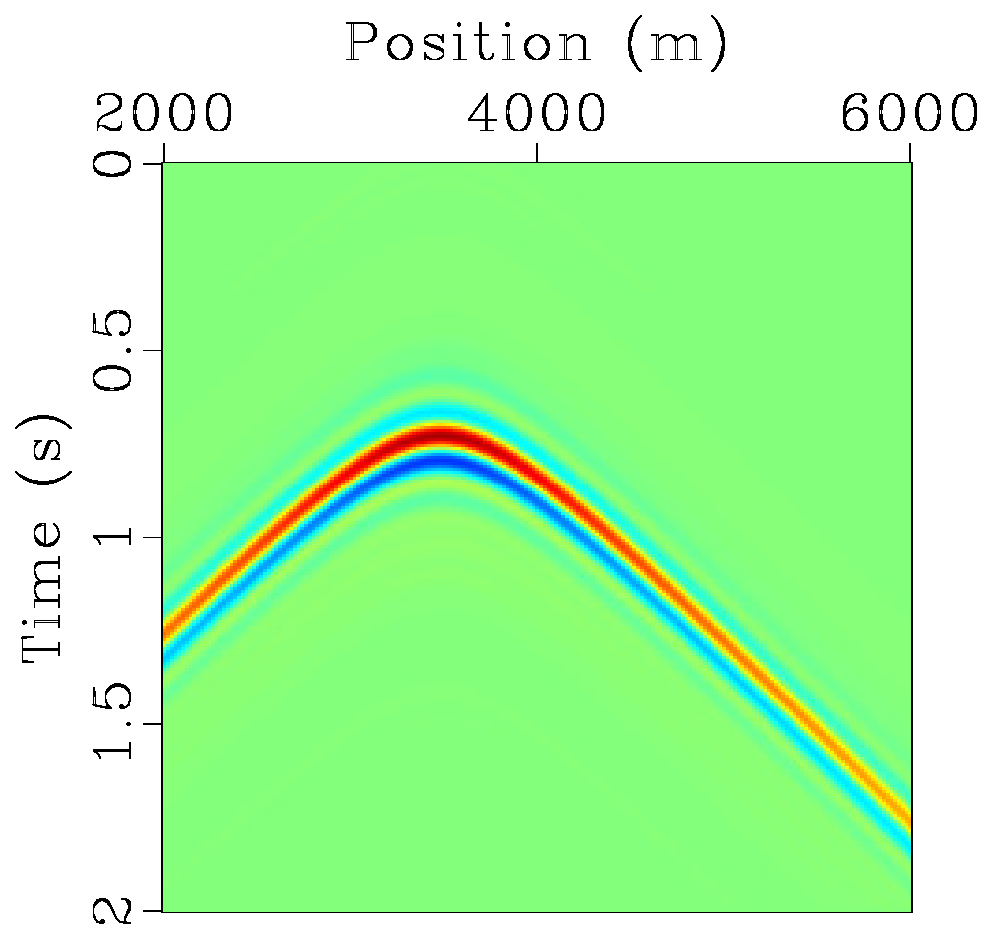
\includegraphics[width=0.32\textwidth]{dsrcphh0.pdf}}
  \subfloat[\label{fig:dfwdplh0}]{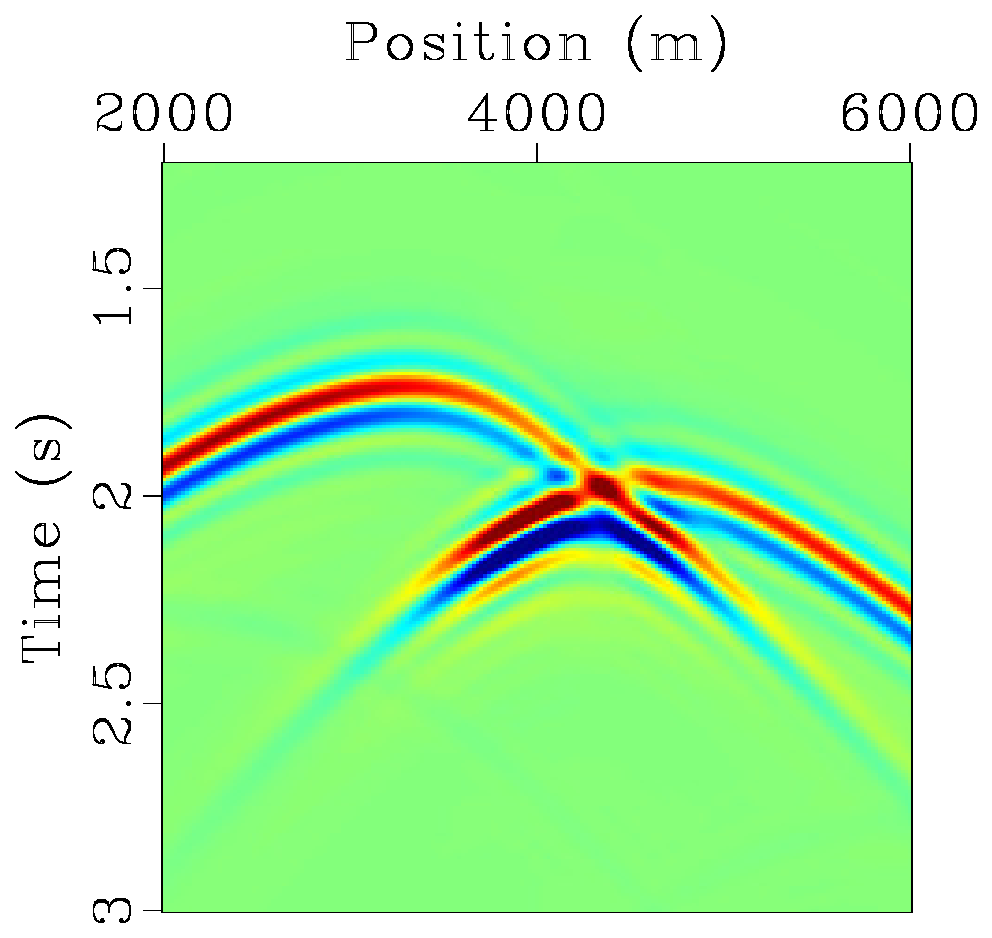
\includegraphics[width=0.32\textwidth]{dfwdplh0.pdf}}
  \caption{Data generated using configuration in Figure
    \ref{fig:olensrays0}. (a) traces from point source at $(3500,3500)$
    with $[1, 2, 7.5, 12.5]$ Hz zero phase trapezoidal bandpass
    filter wavelet, delayed by $0.5$ s. (b) Equivalent extended source on
    the source surface at depth $z_s=3000$ m. (c) Gather generated by
    equivalent source shown in (b). Color scale is same for (a) and (c).}
\end{figure}

The second example is intended as a cartoon of long-offset node
acquisition. It features a depth-dependent increasting
velocity. Figure \ref{fig:ooplrays0} shows bulk modulus field (once again, the
density is constant and $= 1$ g/cm$^3$). The source and receiver
surfaces are horizontal lines, as in the first example, at depths
$z_s=500$ m and $z_r= 100$ m respectively. A point source used to
generate a data traces is positioned at $z_s=500, x_s=10000$ m. The
source wavelet is the same bandpass filter as in
the previous example.

\begin{figure}
  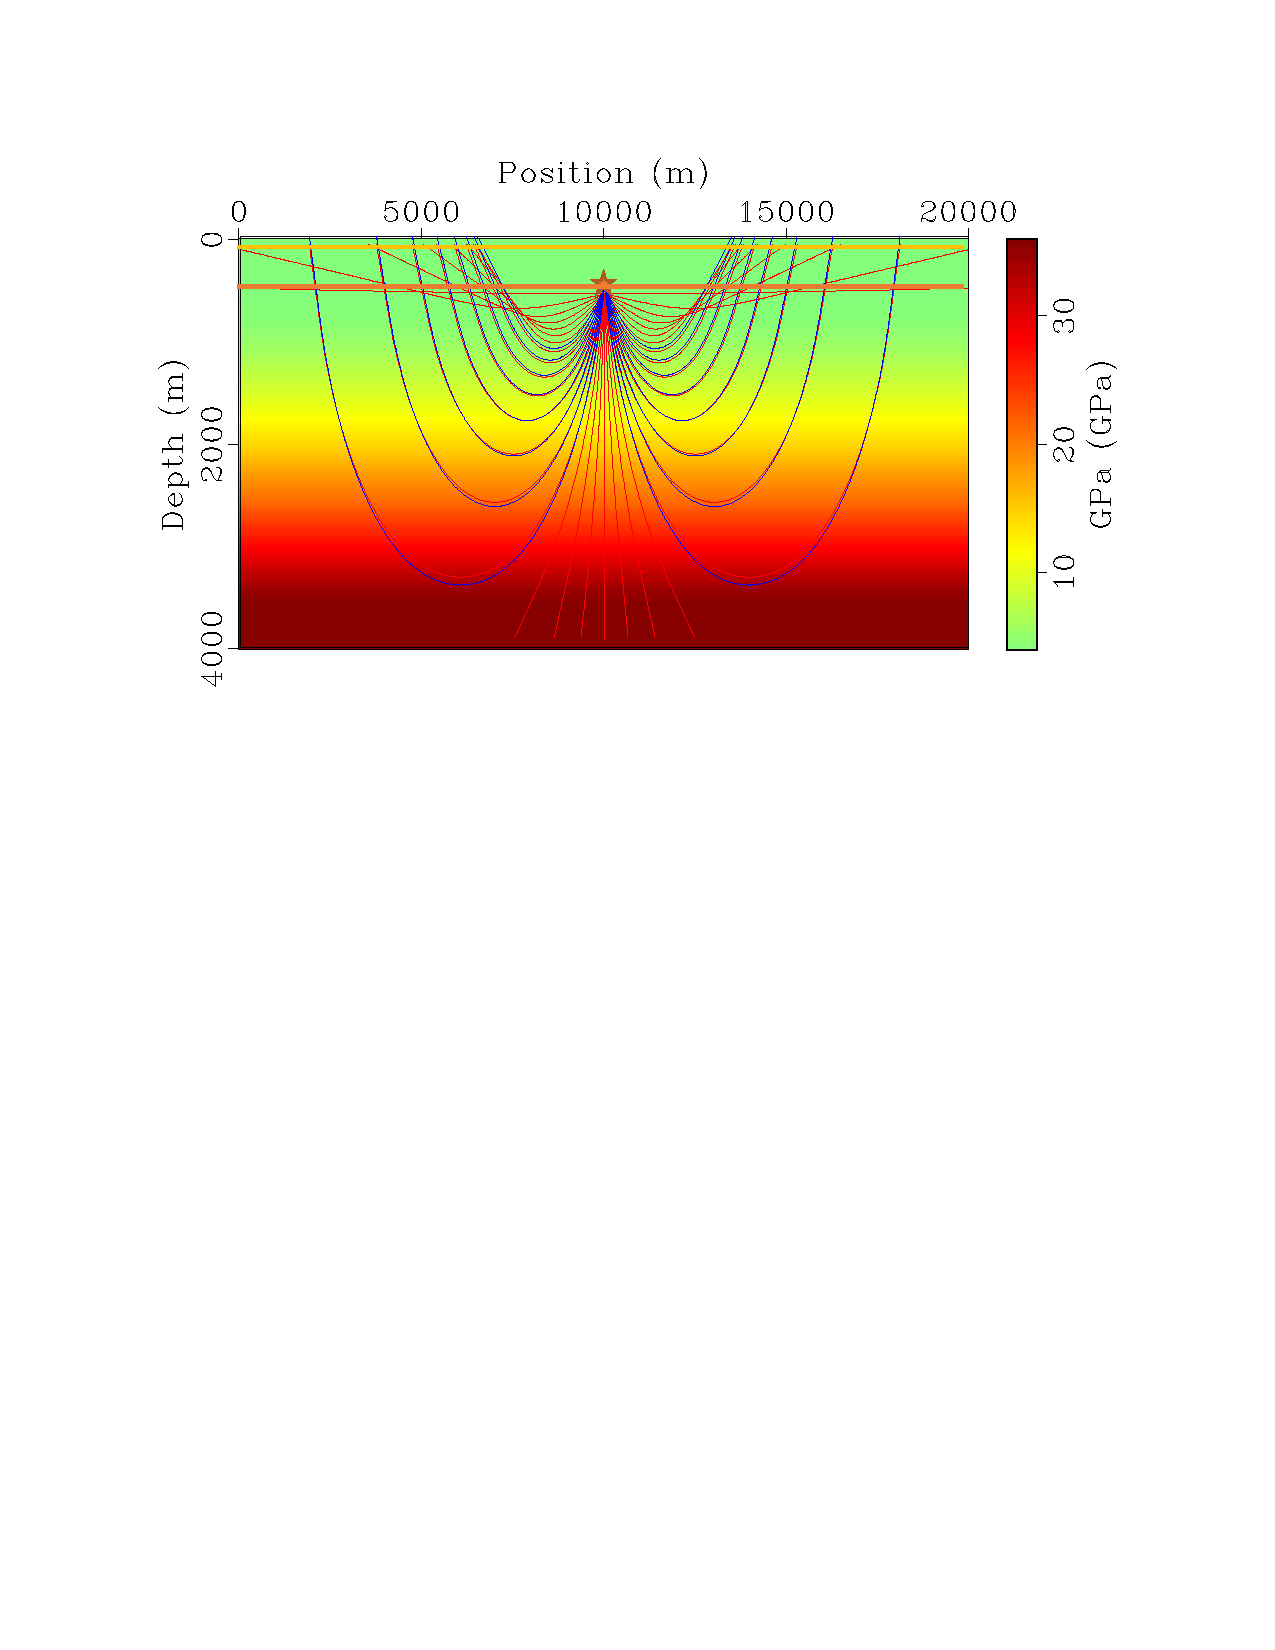
\includegraphics[width=\textwidth]{ooplrays0.pdf}
  \caption{Bulk modulus generating diving waves. Color scale unit is
    GPa. Orange horizontal line is source surface at depth $z_s= 500$
    m, yellow horizontal
    line is receiver surface at depth $z_r=100$ m. Point source location for data
    generation at $(500, 10000)$ m indicated with star. Overlain with rays from point
    source to receiver surface.}
  \label{fig:ooplrays0}
\end{figure}


A diving wave arrival is clearly visible in Figure
\ref{fig:ndwraw0}, which displays data traces over the position range $14000 \le
x_r \le 20000$ m. The ray field connecting the point source to the
receiver surface is plotted with the diving rays in blue, the rest in
red. Note that at the source, the diving rays are incoming if the
orientation is chosen with inwards = down, in contrast to the previous
example, while they are outgoing at
the receiver surface if it is oriented so that inwards = down also.

This geometry permits inversion of the diving wave data alone, which
is isolated via a mute, depicted in (Figure \ref{fig:ndwmute0}. The
mute includes time truncation at 6 s, and offsets between -10000 and
10000 m. The isolated
diving wave (window between offsets 4000 and 10000) is shown in
Figure \ref{fig:ndwdata0}. 


\begin{figure}
  \centering
  \subfloat[\label{fig:ndwraw0}]{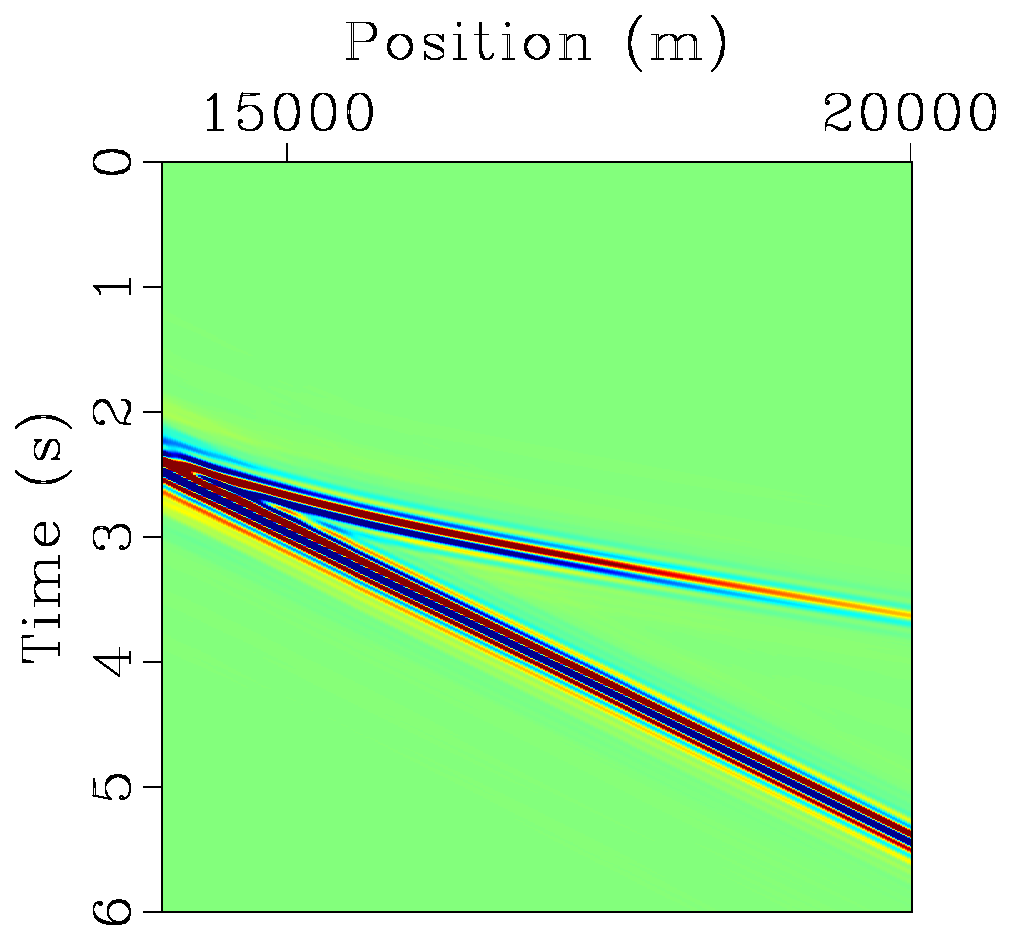
\includegraphics[width=0.32\textwidth]{ndwraw0.pdf}}
  \subfloat[\label{fig:ndwmute0}]{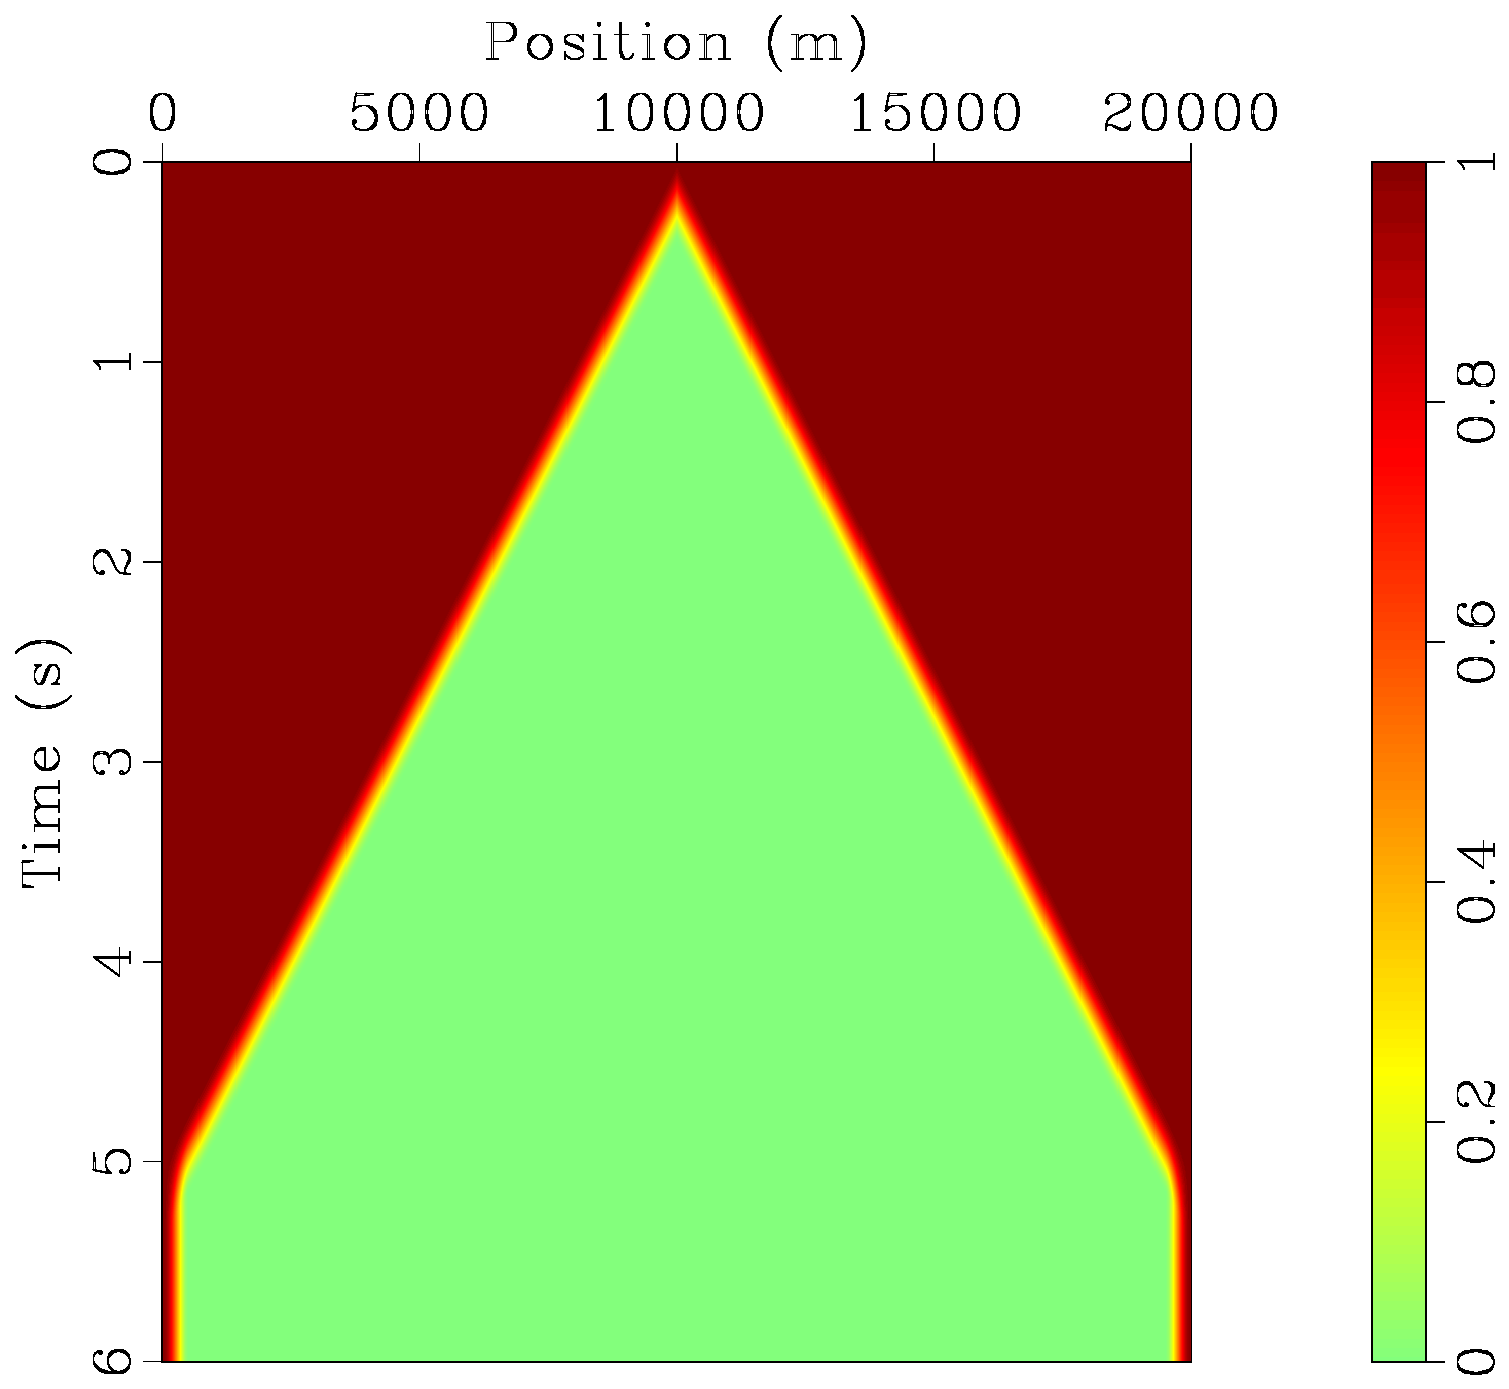
\includegraphics[width=0.32\textwidth]{ndwmute0.pdf}}
  \subfloat[\label{fig:ndwdata0}]{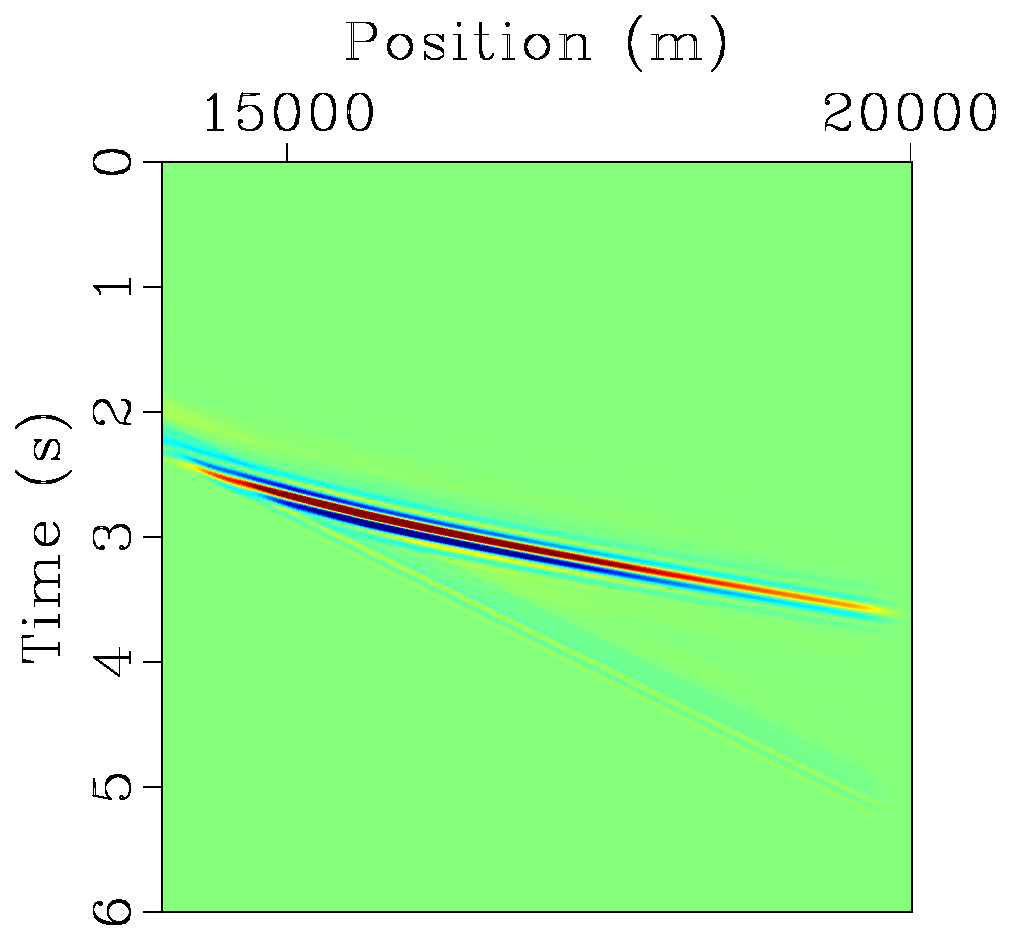
\includegraphics[width=0.32\textwidth]{ndwdata0.pdf}}
  \caption{Data generated using configuration in Figure
    \ref{fig:ooplrays0}. (a) traces from point source at $(500,10000)$ m
    with $[1, 2, 7.5, 12.5]$ Hz zero phase trapezoidal bandpass
    filter wavelet, delayed by $0.4$ s. (b) Mute function,
    incorporated in the sampling operator $P_r$. (c) Diving wave
    gather. Color scale is same for (a) and (c).}
\end{figure}
%As explained in the Introduction, the downgoing constraint on the square-integrable
%source functions $h_s, f_s$ is
%essential both for finite energy solutions of the system
%\ref{eqn:awepm} to exist, and for these solutions to have well-defined
%traces on the receiver surface $z=z_r$. This constraint will be
%assumed throughout, often tacitly.
%For downgoing solutions of system \ref{eqn:awepm}, the key
%components ($p^{\pm}$ and $v^{\pm}_z$) are continuous functions of $z$
%in the open slab $z_s<z<z_r$ with well-defined limits at the boundary
%planes, but may be discontinuous at the source plane
%$z=z_s$. Similarly, the roles of $z_s$ and $z_r$ will be interchanged
%in some of the constructions to come, and the corresponding solutions
%may be discontinuous at $z=z_r$. Accordingly, interpret $P_s$, $P_r$
%as the limit from right and left respectively: for $u=p^{\pm}$ or
%$v^{\pm}_z$,
%\begin{eqnarray}
 % \label{eqn:defsamp}
 % P_su(x,y,t) &=& \lim_{z \rightarrow z_s^+} u(x,y,z,t),\nonumber \\
 % P_ru(x,y,t) &=& \lim_{z \rightarrow z_r^-} u(x,y,z,t).                  
%\end{eqnarray}



%\noindent {\bf Remark:} To connect with the formulation presented in
%the introduction, note that for continuous $u$,
%$P_su(x,y,t)=u(x,y,z_s,t)$, and therefore the adjoint of $P_s$ (in the
%sense of distributions) is $P_s^Th(x,y,z,t) =
%h(x,y,t)\delta(z-z_s)$. Write ${\cal P}_s = \mbox{diag }(P_s,P_s)$ and
%similarly for ${\cal P}_r$. Then
%\[
 % {\cal S}^{+}_{z_s,z_r} = {\cal P}_r L^{-1}({\cal P}_s)^T,
%\]
%in which $L^{-1}$ is interpreted in the causal sense, and similarly
%for ${\cal S}^{-}$. Sources confined to $z=z_s$ are precisely those
%functions (distributions, really) output by ${\cal P}_s^T$, so the
%problem statements \ref{eqn:esi} and \ref{eqn:esis} can be rewritten
%in terms of ${\cal S}^+_{z_s,z_r}$, with $P$ identified with ${\cal P}_r$.

%${\cal S}^{\pm}$ is not stably invertible: its columns are
%approximately linearly dependent, as will be verified below. The
%diagonal components of ${\cal S}^{\pm}$ thus carry essentially all of
%its information, and it is in terms of these that a sensible inverse problem
%is defined.

\section{Time Reversal}

Recall that the source vector $(h_s,f_s)$ is assumed to produce a
downgoing field $(p^+,\bv^+)$, that is, emanates high-frequency energy only along
rays that make an angle with the vertical bounded below by a common
minimum angle. Such rays leave $\Omega$ within a common maximum
time. Consequently (Appendix B), in the
slab $z_s<z<z_r$, the field $(p^+,\bv^+)$ approximates the solution of an
anti-causal evolution equation. Choose $\chi(t)$ to be a smooth function
that is $= 0$ for $t \gg 0$ and $=1$ at times when near rays carrying
high-frequency energy in $(p^+,\bv^+)$ cross $z=z_r$. Define 
$(\tilde{p}^-,\tilde{\bv}^-)$ to be the solution in the half-space
$\Omega \times \bR$ of
\begin{eqnarray}
\label{eqn:revawe}
  \frac{1}{\kappa}\frac{\partial \tilde{p}^-}{\partial t} & = & - \nabla \cdot \tilde{\bv}^-, \nonumber \\
  \rho\frac{\partial \tilde{\bv}^-}{\partial t} & = & - \nabla \tilde{p}^-,\nonumber \\
  \tilde{p}^- & =& 0,  \mbox{ for } t \gg 0\\ 
  \tilde{\bv}^- & = & 0 \mbox{ for } t \gg 0\\
  P_r\tilde{p}^- &=& \chi P_rp^+ . 
\end{eqnarray}
That is, $\tilde{p}^-$ has the same boundary value on $z=z_r$ as
$p^+$, except for low-frequency residue that is muted by
$\chi$. Therefore
$p^+ \approx \tilde{p}^-, \bv^+ \approx \tilde{\bv}^-$ near
$z=z_r$. Since the right-hand sides in the system \ref{eqn:awepm} are
singular only on $z=z_s$, and the high-frequency components of
$(p^+,\bv^+)$ are carried by downgoing rays, these differ negligibly
from the the high-frequency components of
$(\tilde{p}^-,\tilde{\bv}^-)$ in the space-time slab $z_s<z<z_r$, and
the approximation holds throughout this region. In particular
$P_sv^+_z \approx P_s \tilde{v}^-_z$. In view of the relation
\ref{eqn:tracejump10},
\begin{equation}
  \label{eqn:tildevtohsubs}
  -2P_s\tilde{v}^-_z \approx h_s,
\end{equation}
so solution
of the system \ref{eqn:revawe} followed by restriction to $z=z_s$ and
multiplication by $-2$ 
approximately inverts the map $S^+_{z_s,z_r}: h_s \mapsto P_rp^+$.

Next observe that in view of the relation \ref{eqn:tracejump20}, and
the downgoing nature of the ray system carrying the high frequency
energy in $(p^+,\bv^+)$, the field $(\tilde{p}^-,\tilde{\bv}^-)$ is
actually the restriction to $z<z_r$ of the anti-causal solution of \ref{eqn:awepm}
with $z_s$ replaced by $z_r$, zero constitutive defect, and vertical
load given by the jump in pressure at $z=z_r$ - for this field, use
the same notation. Continuity of vertical
velocity $\tilde{v}^-_z$ at $z=z_r$ implies that the vertical load is
\[
  f_r = -[\tilde{p}^-]|_{z=z_r} =-(\lim_{z\rightarrow
    z_r^+}\tilde{p}^- - \lim_{z\rightarrow
    z_r^-}\tilde{p}^-)
\]
\[
  \approx 2 P_r \tilde{p}^- = 2 P_r p^+
\]
(from the definition \ref{eqn:defsamp}, $P_r$ is the limit from the
left). Thus
\[
  P_s \tilde{v^-_z} \approx V^-_{z_r,z_s}(2 P_rp^+) \approx
  2V^-_{z_r,z_s}S^+_{z_r,z_s}h_s.
\]
so
\[
  h_s \approx -2 P_s v^+_z \approx -2 P_s \tilde{v}^-_z \approx
  -4V^-_{z_r,z_s}S^+_{z_r,z_s}h_s
\]
Combine this observation with \ref{eqn:tildevtohsubs} to obtain
\[
 -4  V^-_{z_r,z_s} S^+_{z_s,z_r}  \approx  I,
\]
This relation combines with the identity \ref{eqn:trtrcomp} to
yield the first main result of this section:
\begin{eqnarray}
  \label{eqn:approxinv}
  (V^+_{z_s,z_r})^T S^+_{z_s,z_r} & \approx & \frac{1}{4}I, \nonumber\\
  (S^+_{z_s,z_r})^T V^+_{z_s,z_r} & \approx & \frac{1}{4}I, \nonumber\\
  V^+_{z_s,z_r} (S^+_{z_s,z_r})^T & \approx & \frac{1}{4}I, \nonumber\\
  S^+_{z_s,z_r} (V^+_{z_s,z_r})^T & \approx & \frac{1}{4}I.
\end{eqnarray}.
The second equation is simply the transpose of the first, and the
last two follow by by an exactly analogous argument using time
reversal and interchange of the roles of $z_s$ and$z_r$.

The conclusion is significant enough to merit restating in English:
provided that high-frequency energy in the various fields is carried
along downgoing ray fields, the transpose of $V^+$ is an approximate
inverse to $S^+$, modulo a factor of 4. To recover the pressure source
$h_s$ generating a pressure gather $P_rp$ at $z=z_r$, multiply the
latter by -2, then apply the transpose of $V^+_{z_s,z_r}$ to this
gather, reading out a vertical velocity field at $z=z_s$. Multiply
again by -2 and you have a high-frequency approximation to $h_s$.



It follows from the adjoint state method (see Appendix A for details) that
\begin{equation}
  \label{eqn:sadj1}
  ({\cal S}^{\pm}_{z_s, z_r})^T = -{\cal S}^{\mp}_{z_r,z_s}
\end{equation}

Define $R$ to be the {\em time-reversal operator} on functions of
space-time, $Rf(\bx,t) = f(\bx,-t)$, and ${\cal R}$ to be the {\em
  acoustic field time-reversal operator}
\begin{equation}
  \label{eqn:trdef}
  {\cal R} \left(
    \begin{array}{c}
      p\\
      \bv
    \end{array}
  \right) =
  \left(
    \begin{array}{c}
      Rp\\
      -R\bv
    \end{array}
  \right)
\end{equation}
Then 
\begin{equation}
  \label{eqn:trsadj}
  {\cal R}{\cal S}^{\mp} = -{\cal S}^{\pm}_{z_r,z_s}{\cal R}
\end{equation}
Since $R^2 = I$ and ${\cal R}^2 = I$, the identities \ref{eqn:sadj1} and \ref{eqn:trsadj} imply that
\begin{equation} 
  \label{eqn:trtr}
 ({\cal S}^{\pm}_{z_s,z_r})^T = {\cal R}{\cal S}_{z_r,z_s}^{\pm}{\cal R}=
 -{\cal S}^{\mp}_{z_r,z_s}.
\end{equation}
The relation \ref{eqn:trtr} implies that
\begin{eqnarray}
  (S^{\pm}_{z_s,z_r})^T &=& -S^{\mp}_{z_r,z_s} \nonumber\\
                        &=& R S^{\pm}_{z_r,z_s}R, \nonumber\\
    (V^{\pm}_{z_s,z_r})^T &=& -V^{\mp}_{z_r,z_s} \nonumber\\
                        &=& R V^{\pm}_{z_r,z_s}R.
                            \label{eqn:trtrcomp}
\end{eqnarray}




\section{Pressure-to-Source}

Since the system \ref{eqn:awepm} has a unique solution by standard
theory \cite[]{Lax:PDENotes}, the source vector field $(h_s,f_s)$
determines the acoustic field $(p^{\pm},\bv^{\pm})$ in space time, and
in particular the limits from the right at $z=z_s$, $P_sp^{\pm}$ and
$P_sv_z^{\pm}$. This relation is not invertible: it is not possible to
prescribe both pressure and normal velocity on a surface such as
$z=z_s$. So the columns of the matrix operator
${\cal S}^{\pm}_{z_s,z_r}$ must satisfy a linear relation. In this
section I will explain this relation; it involves the {\em
  pressure-to-source} map. This operator also turns out to be the
principal component of a preconditioning strategy for iterative
solution of the optimization problem \ref{eqn:esis}, so I will devote
some effort to its proper definition. It is closely related to the
Dirichlet-to-Neumann operator mentioned in the introduction.

While it is not possible to prescribe both pressure and velocity on
$z=z_s$ in solutions of \ref{eqn:awepm}, it is possible to
prescribe pressure only, for instance: if the function $\phi$ on
the surface $z=z_s$ satisfies suitable conditions, for
example the downgoing constraint mentioned earlier, a unique solution
exists for the acoustic system in both half-spaces $\pm z > z_s$:
\begin{eqnarray}
\label{eqn:awe0}
  \frac{1}{\kappa}\frac{\partial p_{\pm}}{\partial t} & = & - \nabla \cdot \bv_{\pm}, \nonumber \\
  \rho\frac{\partial \bv_{\pm}}{\partial t} & = & - \nabla
                                                    p_{\pm}, \nonumber \\
  p_{\pm} & =& 0,  \mbox{ for } t \ll 0, \nonumber\\ 
  \bv_{\pm} & = & 0 \mbox{ for } t \ll 0, \nonumber\\
  \lim_{z \rightarrow z_s^{\pm}}p_{\pm}(x,y,t,z)& =& \phi(x,y,t).
\end{eqnarray}
Note that the subscript $\pm$ here refers to the sign of $z-z_s$, as opposed
to the superscript ${\pm}$, which refers to the sign of $t$ throughout
this paper.

From the boundary condition (last equation in \ref{eqn:awe0}), one
sees that the pressures $p_{\pm}$ in the two half-spaces have the same
limit at the boundary $z=z_s$. Stick the two half-space
solutions together to form an acoustic field $(p^+,\bv^+)$ in all of
space-time, that is,
\begin{equation}
  \label{eqn:awealt}
  p^+(x,y,z,t) =
  \left\{
    \begin{array}{c}
      p_+(x,y,z,t) \mbox{ if } z>0,\\
      p_-(x,y,z,t) \mbox{ if } z<0,
    \end{array}
  \right.
\end{equation}
and a similar definition for $\bv^+$. Then $p^+$ is continuous across
$z=z_s$, and the boundary condition in system \ref{eqn:awe0} may be
written as $P_sp^+=\phi$.

The same construction can be carried out in the anti-causal sense,
with anti-causal half-space solutions glued together to form a
full-space distribution solution $(p^-,\bv^-)$, with the property that
$p^-$ is continuous across $z=z_s$ and $P_sp^-=\phi$.

The reader may object that the notation $(p^\pm,\bv^\pm)$ is already in
use, for the solution of \ref{eqn:awepm}. This objection is
valid. However, {\em in the sense
  of distributions}, $(p^{\pm},\bv^{\pm})$ as defined in display
\ref{eqn:awealt}, is {\em exactly} the causal solution of \ref{eqn:awepm}
for the choice $h_s = -[v^{\pm}_{z}]|_{z=z_s}, f_s=0$, as follows from a
simple integration-by-parts calculation. So the notation is consistent!

The negative jump $-[v^{\pm}_{z}]|_{z=z_s}$ is thus a function of $\phi$. Define
the {\em pressure-to-source} operator $\Lambda^{\pm}_{z_s}$ by
\begin{equation}
  \label{eqn:deflam}
  \Lambda^{\pm}_{z_s}\phi = -[v^{\pm}_{z}]|_{z=z_s}
\end{equation}
The conclusion: if $h_s = \Lambda^{\pm}_{z_s}\phi$ and $f_s=0$ in the
system \ref{eqn:awepm}, then $\phi=P_sp^{\pm}$.

Otherwise put, $S^{\pm}_{z_s,z_s}\Lambda^{\pm}_{z_s} \phi = \phi$, so
$\Lambda^{\pm}_{z_s}$ is inverse to $S^{\pm}_{z_s,z_s}$. The relation
\ref{eqn:trtrcomp} implies in turn that
\begin{equation}
  \label{eqn:lamadj}
  (\Lambda^{\pm}_{z_s})^T = - \Lambda^{\mp}_{z_s}
\end{equation}

There is also a {\em velocity-to-source} operator. For the solution
$(p^{\pm},\bv^{\pm})$ of system \ref{eqn:awepm} with $h_s=0$, the
normal component of velocity, $v^{\pm}_z$, is continuous across
$z=z_s$, and the velocity source (vertical load)
$f_s=-[p^{\pm}]_{z=z_s}$. I will not name the velocity-to-source
operator, as it does not appear explicitly in the developments to
follow. As will be seen, it is essentially the inverse of the
pressure-to-source operator.

The quadratic form defined by $\Lambda^{\pm}_{z_s}$ has fundamental
physical significance. Define the total acoustic energy $E^{\pm}(t)$ of the
field $(p^{\pm},\bv^{\pm})$, at time $t$ by
\begin{equation}
  \label{eqn:defae0}
  E^{\pm}(t) = \frac{1}{2} \int \,d\bx \, \left(\frac{(p^{\pm})^2}{\kappa} + \rho |\bv^{\pm}|^2\right)(\bx,t).
\end{equation}
Then
\begin{equation}
  \label{eqn:elim}
  \pm \lim_{\pm t \rightarrow \infty} E^{\pm}(t) =  \langle P_sp^{\pm},
  (\Lambda^{\pm}_{z_s} P_sp^{\pm}) \rangle_{L^2(z=z_s)}.
\end{equation}
That is, the value of the quadratic form defined by
$\Lambda^{\pm}_{z_s}$, evaluated at the pressure trace on $z=z_s$,
gives the total energy transferred from the source to the
acoustic field over time. Since $E$ is itself a positive definite
quadratic form in the acoustic field, it follows that $\pm
\Lambda^{\pm}_{z_s}$ is positive semi-definite. 

While $\Lambda^{\pm}_{z_s}$ is positive semi-definite, it is not
symmetric. However, it is {\em approximately symmetric} in the
high-frequency sense. This fact follows from a
geometric optics analysis of the half-space solution. This leads to
the identification of $\Lambda^{\pm}_{z_s}$ as a {\em
  pseudodifferential operator} of order zero on $z=z_s$, with principal symbol
\begin{equation}
  \label{eqn:lamsym}
  \sigma_0(\Lambda^{\pm}_{z_s}) = \pm 2(\kappa(\bx)
  \rho(\bx))^{1/2}\left(1-\frac{\kappa(\bx)(\xi^2+\eta^2)}{\rho(\bx)\omega^2}\right)^{-1/2}.
\end{equation}
Here $\xi$, $\eta$, and $\omega$ are the dual Fourier variables to
$x$, $y$, and $t$ respectively. The downgoing assumptions means that
for local planewave components of $P_sp$, the quantity inside the
square root is positive. Thus $\Lambda^{\pm}_{z_s}$ has real principal
symbol (in fact, the entire symbol is real) hence defines an
asymptotically symmetric operator:
\begin{equation}
  \label{eqn:lamappsim}
  (\Lambda^{\pm}_{z_s})^T \approx \Lambda^{\pm}_{z_s}.
\end{equation}
(For more on this, see \cite{StefUhl:05}.)
The analysis also reveals that the solution components not continuous
at $z=z_s$ are odd there:
\begin{equation}
  \label{eqn:odd1}
  \lim_{z\rightarrow z_s^+} v^{\pm}_{z} \approx - \lim_{z\rightarrow z_s^-}
  v^{\pm}_{z}
\end{equation}
for the solution of \ref{eqn:awepm} with $f_s=0$.
Similarly, 
\begin{equation}
  \label{eqn:odd2}
  \lim_{z\rightarrow z_s^+} p^{\pm}\approx - \lim_{z\rightarrow z_s^-}
  p^{\pm}
\end{equation}
for the solution of \ref{eqn:awepm} with $h_s=0$. Here ``$\approx$''
means in the sense of high frequency asymptotics, that is, that the
difference between the two sides is relatively smooth, hence small if
the data is highly oscillatory. Therefore if $f_s=0$ in system \ref{eqn:awepm},
\begin{equation}
  h_s = \Lambda^{\pm}_{z_s}P_sp^{\pm} = -[v^{\pm}_{z}]|_{z=z_s} \approx -2
  P_sv^{\pm}_{z}
  \label{eqn:tracejump10}
\end{equation}
Similarly, if $h_s=0$ in system \ref{eqn:awepm}, then
\begin{equation}
  \label{eqn:tracejump20}
  f_s = -[p^{\pm}]|_{z=z_s} \approx -2 P_s p^{\pm}.
\end{equation}
Thus $f_s$ determines approximately the boundary value of $p^{\pm}$,
as a solution of the acoustic wave system in the half-space
$z>z_s$. However, as repeated in equation \ref{eqn:tracejump10}, a
solution with this boundary value is also the restriction to $z>z_s$
of a solution to \ref{eqn:awepm} with $f_s=0$ and $h_s=
\Lambda^{\pm}_{z_s}P_sp^{\pm}$. Therefore if
\begin{equation}
  \label{eqn:hfcondn}
  h_s =-\frac{1}{2}\Lambda^{\pm}_{z_s}f_s,
\end{equation}
then the pressure boundary value $P_sp^{\pm}$ is the
same for the solutions of \ref{eqn:awepm} for source vectors $(h_s,0)$
and $(0,f_s)$. Since the pressure boundary values are the same, the solutions
in $z>z_s$ are the same. In particular, since $z_r>z_s$ and ${\cal
  S}^{\pm}_{z_s,z_r}(h_s,f_s)^T = (P_rp^{\pm},P_rv^{\pm}_z)^T$, it follows
that
\begin{equation}
  \label{eqn:snull}
  {\cal S}^{\pm}_{z_s,z_r}\left(\frac{1}{2}\Lambda^{\pm}_{z_s}f_s,f_s\right)^T \approx 0.
\end{equation}

Equation \ref{eqn:snull} states the relation between the columns of $
{\cal S}^{\pm}_{z_s,z_r}$ mentioned in the introduction to this
section.



\section{Unitarity}

The next chapter in this story recognizes the relations in display
\ref{eqn:approxinv} as asserting the approximate unitarity of
$S^+_{z_s,z_r}$.

The matrix identity \ref{eqn:snull} implies a relation between $S, V,$
and $\Lambda$ of some interest in itself. After minor re-arrangement, the second row of reads
\begin{equation}
  \label{eqn:snull2}
-\frac{1}{2}\Pi_1{\cal S}^{\pm}_{z_s,z_r}\Pi_0^T\Lambda^{\pm}_{z_s}  \approx
V^{\pm}_{z_s,z_r}.
\end{equation}
In these relations, the projection on the left picks out the vertical velocity component
of a downgoing wavefield at $z=z_r$: that is,
\[
-\frac{1}{2}\Pi_1{\cal S}^{\pm}_{z_s,z_r}\Pi_0^T\Lambda^{\pm}_{z_s}P_sp^+
=-\frac{1}{2}P_r v_z^+,
\]
where $(p^+, \bv^+)$ solve the system \ref{eqn:awepm} with $f_s=0$ and
$h_s = \Lambda^{\pm}_{z_s}P_sp^+$. On the other hand, from relation
\ref{eqn:tracejump10},
\[
  P_r v_z^+ = -\frac{1}{2}\Lambda^+_{z_r}P_r p^+
\]
where
\[
  P_r p^+ = \Pi_0{\cal S}^{+}_{z_s,z_r}\Pi_0^T\Lambda^{+}_{z_s}P_s
  p^+
\]
\[
  = S^+_{z_s,z_r}\Lambda^{+}_{z_s}P_sp^+
\]
Therefore combining the last two equations with \ref{eqn:snull2},
obtain
\begin{equation}
  \label{eqn:sv}
  \frac{1}{4}\Lambda^+_{z_r}S^+_{z_s,z_r}\Lambda^{+}_{z_s} = V^+_{z_s,z_r}.
\end{equation}
This is the promised relation.


As shown in the last section, $4(V_{z_s,z_r}^+)^T$ is approximately
inverse to $S^{+}_{z_s,z_r}$. Therefore, transposing both sides of
equation \ref{eqn:sv} and using \ref{eqn:approxinv}, obtain
\begin{equation}
  \label{eqn:almostunitary}
  4(V_{z_s,z_r}^+)^TS^+_{z_s,z_r} = [ (\Lambda^+_{z_s})^T
  (S^{+}_{z_s,z_r})^T(\Lambda^+_{z_r})^T]S^{+}_{z_s,z_r} \approx I.
\end{equation}

The remarkable feature of the identity \ref{eqn:almostunitary} is that
it exhibits an approximate right inverse of $S^+$ as an adjoint with
respect to a weighted inner product - or it would, if the operators
$(\Lambda^+)$ were symmetric positive definite. As noted earlier,
these operators are only approximately symmetric, though they are
positive semi-definite. That is not a great obstacle, however:
symmetrizing them in the obvious way commits a negligible error, of
the sort that this paper already neglects wholesale. That is,
\begin{equation}
  \label{eqn:unitary}
  [ \frac{1}{2}((\Lambda^+_{z_s})^T+ \Lambda^+_{z_s})
  (S^{+}_{z_s,z_r})^T \frac{1}{2}((\Lambda^+_{z_r})^T+
  \Lambda^+_{z_r})]S^{+}_{z_s,z_r} \approx I.
\end{equation}


The symmetrized $\Lambda$ operators are at least positive
semi-definite, hence define (at least) semi-norms.
Similar relations have been derived for other scattering operators,
and have been used to accelerate iterative solutions of inverse
scatering problems: \cite{DafniSymes:SEG18b} review some of this
literature.

\section{Accelerated Iterative Inversion}

For convenience, in this section write $S$ in place of
$S^+_{z_s,z_r}$. Also abbreviate the symmetrized $\Lambda$ operators
using notation suggesting weight
operators in model and data spaces:
\begin{eqnarray}
  W_m^{-1}&=& \frac{1}{2}((\Lambda^+_{z_s})^T+
              \Lambda^+_{z_s}),\nonumber \\
  W_d &=& \frac{1}{2}((\Lambda^+_{z_r})^T+ \Lambda^+_{z_r}).
          \label{eqn:wdef}
\end{eqnarray}
The identification of the symmetrized $\Lambda^+_{z_s}$ as the inverse
of another operator $W_m$ is formal, since the former operator is
likely to have null (or nearly-null) vectors due to aperture-related
amplitude loss. Since some version of $W_m$ is essential in the
formulation for effective preconditioning, I will derive a usable
candidate to stand in for it below.

Adopting Hilbert norms defined by the operators $W_m$ and $W_d$ in its
domain and range respectively, the adjoint of $S$ is given by
\begin{equation}
\label{eqn:wadj}
S^{\dagger} = W_m^{-1}S^TW_d,
\end{equation}

In this notation, the relation \ref{eqn:unitary} takes the form
\begin{equation}
  \label{eqn:wunitary}
  S^{\dagger}S \approx I.
\end{equation}
That is to say, $S$ is approximately unitary with respect to the
weighted norms defined by $W_m$ and $W_d$. Therefore a Krylov space
method employing these norms will converge rapidly, at least for the
well-determined components of the solution.

The most convenient arrangement the Conjugate Gradient (CG) algorithm
taking advantage of the structure \ref{eqn:wadj} is the {\em
  Preconditioned CG}. Allowing that the fit error will be measured by
the data space norm, the least squares problem to be solved is not
just $Sh \approx d$, but a regularized version:
\begin{equation}
  \label{eqn:einv}
  \mbox{minimize}_h \|Sh-d\|^2_d + \alpha^2 \|Ah\|^2_m
\end{equation}

\noindent {\bf Remark:} recall that the modified data space norm $\|d\|_d^2 = \langle
d, W_d d\rangle$ has physical meaning: for acoustics, it is
proportional to the power transmitted to the fluid by the source.

The minimizer of the objective defined in equation \ref{eqn:einv}
solves the normal equation
\begin{equation}
  \label{eqn:norm0}
  (S^{\dagger}S + \alpha^2 A^{\dagger}A)h = S^{\dagger}d 
\end{equation}
where the weighted adjoint $S^{\dagger}$ has already been defined in equation \ref{eqn:wadj}, and $A^{\dagger}$ is the adjoint of $A$ in the weighted model space norm defined by $W_m$, namely
\begin{equation}
  \label{eqn:aadj}
  A^{\dagger} = W_m^{-1}A^TW_m.
\end{equation}

Note that the normal operator appearing on the left-hand side of
\ref{eqn:norm0} is not an approximate identity, due to the presence of
the regularization term: the spectrum increases in spread with
increasing $\alpha$, leading to slower convergence. Fortunately for
the present setting, the operators $W_m^{-1}$, $A$, and $W_m$
approximately commute (they are scalar {\em pseudodifferential}, once
the difficulties with the definition of $W_m$, mentioned above, are
taken care of). Scalar pseudodifferential operators approximately
commute, so $A^{\dagger} \approx A^T$. Therefore
\begin{equation}
  \label{eqn:normapprox}
  S^{\dagger}S + \alpha^2 A^{\dagger}A \approx I + \alpha^2A^TA
\end{equation}
Recall that $A$ is simply multiplication by the Euclidean distance to
the physical source point $\bx_s$: $A u (\bx) = |\bx-\bx_s|u(\bx),
A^TAu(\bx) = |\bx-\bx_s|^2u(\bx)$. So the equation $(I+\alpha^2
A^TA)u=b$ is trivial to solve, and this is a key characteristic of a
good preconditioner. However this observation must be combined with
the weighted norm structure.

Rewrite the normal equation \ref{eqn:norm0} as
\begin{equation}
  \label{eqn:norm1}
  W_m^{-1}(S^TW_dS + \alpha^2 A^TW_mA)h = W_m^{-1}S^TW_md 
\end{equation}
Since $W_m$ is self-adjoint and positive semidefinite, the common factor on both sides of \ref{eqn:norm1} can be re-written as
\begin{equation}
  \label{eqn:normpart}
  Nh = (S^*S + \alpha^2 A^*A)h = S^*d 
\end{equation}
in which $S^*, A^*$ are the adjoints with the original (Euclidean)
inner product in the domains but the weighted inner product in data
space:
\begin{eqnarray}
  \label{eqn:sadjwt}
  S^* &=& S^T W_d,\\
  A^* &=& A^T W_m.
\end{eqnarray}
Note the $S^*S$ and $A^*A$ are symmetric in the Euclidean sense, so
equation \ref{eqn:normpart} is a symmetric positive (semi-)definite
linear system, just the sort of thing for which the 
The Preconditioned Conjugate Gradient (``PCG'') algorithm was
designed. PCG for solution
of equation \ref{eqn:normpart} with preconditioner $M$ is usually
written as Algorithm 1 (see for example \cite{Golub:2012}):

\begin{algorithm}[H]
\caption{Preconditioned Conjugate Gradient Algorithm, Standard Version}
\begin{algorithmic}[1]
\State Choose $h_0=0$ 
  \State $r_0 \gets S^*d$
  \State $p_0 \gets M^{-1} r_0$
  \State $g_0 \gets p_0$
  \State $q_0 \gets Np_0$
  \State $k \gets 0$
  \Repeat
  \State $\alpha_k \gets \frac{\langle g_k,r_k \rangle}{\langle p_k,q_k\rangle}$
  \State $h_{k+1} \gets h_k + \alpha_k p_k$
  \State $r_{k+1} \gets r_k - \alpha_kq_k$
  \State $g_{k+1} \gets M^{-1} r_{k+1}$
  \State $\beta_{k+1} \gets \frac{\langle g_{k+1},r_{k+1}\rangle}{\langle g_k,r_k\rangle}$
  \State $p_{k+1}\gets g_{k+1}+\beta_{k+1}p_k$
  \State $q_{k+1} \gets Np_{k+1}$
  \State $k \gets k+1$
  \Until{Error is sufficiently small, or max iteration count exceeded} 
\end{algorithmic}
\end{algorithm}
The iteration converges rapidly if $M^{-1}N \approx I$. This is true
if and only if the symmetrized operator $M^{-1/2}NM^{-1/2} \approx I$,
which is in turn true if the eigenvalues of $M^{-1/2}NM^{-1/2}$ are
close to 1 (actually works well is most of these eigenvalues are close
to 1, and the rest are small - which is the case for the current
problem)..  Further, PCG is computationally effective is M is easy to
invert.

From \ref{eqn:normapprox} and \ref{eqn:norm1}, it follows that
\[
  W_m^{-1}(S^TW_dS + \alpha^2 A^TW_mA) \approx I + \alpha^2 A^TA.
\]
This observation suggests using $M=W_m(I+\alpha^2A^TA)$. This choice
is not symmetric, but since the operators on the right-hand side are
scalar pseudodifferential hence commute, it is equivalent to use of
\begin{eqnarray}
  M         &=&(I+\alpha^2A^TA)^{1/2}W_m(I+\alpha^2A^TA)^{1/2},\nonumber \\
  M^{-1}
            &=&(I+\alpha^2A^TA)^{-1/2}W_m^{-1}(I+\alpha^2A^TA)^{-1/2}.
                \label{eqn:defprecond}
\end{eqnarray}
With this choice, \ref{eqn:normapprox} implies that
$M^{-1}N \approx I$, also $M$ is symmetric. As already mentioned,
powers of $I + \alpha^2A^TA$ are trivial to compute, given the choice
of $A$ made here. We will examine fast algorithms for computing
$W_m^{-1}$ = the symmetrized pressure-to-source operator in the next
section. Note that only $M^{-1}$, hence only $W_m^{-1}$, appears in
Algorithm 1.


\section{Computing and Symmetrizing $\Lambda$}

Computations of $\Lambda^{\pm}_{z_s}$ and its transpose are clearly critical steps in an
implementation of the PCG algorithm outlined in the preceding section.
Direct computation of the pressure-to-source operator $\Lambda^{\pm}_{z_s}$, for instance by solving
\ref{eqn:awepm} and reading off $P_sv^{\pm}_{z}$, turns out to be
numerically ill-behaved. The relation \ref{eqn:snull} provides and
alternative approach, taking advantage of the accurate approximate
inverse to $S^+_{z_s,z_r}$ constructed above. The first row of
\ref{eqn:snull}, slightly rearranged, is
\begin{equation}
  \label{eqn:lamidea}
  \Pi_0{\cal S}^+_{z_s,z_r}\Pi_1^T f_s \approx  -\frac{1}{2} S^+_{z_s,z_r}\Lambda^+_{z_s}f_s.
\end{equation}
The approximate inverse construction for $S^++_{z_s,z_r}$ permits (approximate)
solution of this equation for $\Lambda^+_{z_s}f_s$: apply
$4(V^{+}_{z_s,z_r})^T$ to both sides of equation \ref{eqn:lamidea} and
use the first equation in the list \ref{eqn:approxinv} to get
\begin{equation}
  \label{eqn:lamident}
  \Lambda^+_{z_s} \approx -8(V^{+}_{z_s,z_r})^T\Pi_0 {\cal S}^+_{z_s,z_r}\Pi_1^T.
\end{equation}
This identity is the major result of this section: it shows how
to compute that action of $\Lambda^+_{z_s}$ by propagating the input
pressure trace, identified as a source for the velocity evolution,
forward in time from $z_s$ to $z_r$
reading off the pressure trace on $z=z_r$, identifying it once more as
a point load (source for velocity), propagating it backwards in time from $z_r$ to
$z_s$, and finally reading off the velocity trace, interpreted as a
pressure evolution source on $z_s$. 

The importance of this result lies in the failure of the obvious
method for computing the action of $\Lambda^{\pm}_{z_s}$, namely to
employ the pressure trace as a source in the velocity equation ($f_s$,
in the notation used above) at $z=z_s$, and read off the velocity
field also at $z=z_s$. This difficulty is related to the existence of
tangentially propagating waves and the lack of continuity of the trace
operator. The method implicit in equation \ref{eqn:lamident} avoids
this difficulty by propagating the fields a positive distance in $z$:
assuming as always that the causal fields are downgoing, this step
eliminates any tangentially propagating fields from consideration.


A deeper study of the pressure-to-source operator (or of the closely
related Dirichlet-to-Neumann operator for the second order wave
equation, see \cite{StefUhl:05}) shows that it is approximately
dependent only on the model coefficients near the source surface
($z=z_s$ in this case). Since the homogeneous and lens models are
identical near this surface, it is unsurprising that these figures are
very close to the previous two.  However an even more useful
observation is that the calculations in the approximation
\ref{eqn:lamident} could just as well be carried out in a much smaller
region around the source surface, and produce a result that is
functionally identical in that it will serve as a source for the same
acoustic fields globally, with small error. In effect, equation
\ref{eqn:lamident} involving propagation from source ($z=z_s$) to
receiver ($z=z_r$) surfaces is altered by replacing $z_r$ with a
receiver datum $z_s+\Delta z$ considerably closers to $z_s$:
\begin{equation}
  \label{eqn:lamnear}
  \Lambda^+_{z_s} \approx -8(V^{+}_{z_s,z_s+\Delta z})^T\Pi_0 {\cal
    S}^+_{z_s,z_s+\Delta z}\Pi_1^T.
\end{equation}
Using a receiver datum closer to the source surface has two favorable consequences:
\begin{itemize}
\item The computational domain can be smaller than is necessary to
  simulate the target data, as it need only contain the source
  surface and the receiver datum implicit in
  equation \ref{eqn:lamident}. This shrinkage of the computational
  domain can lead to substantial improvements in computational
  efficiency.
\item Since the receiver data may be chosen much closer to the
  source surface that is the case for the target data, the effective
  aperture active in the relation \ref{eqn:lamident} can be much
  larger, producing an estimated source gather much less affected by
  aperture limitation.
\end{itemize}


As mentioned in the last section, computation of the transpose of
$\Lambda^+$ (exact, not approximate in the high frequency sense) is
critical to the successful construction of the preconditioner. The
relation \ref{eqn:lamident} does not provide a computation for this
operator. However set
\begin{equation}
  \label{eqn:lamtilde}
  \tilde{\Lambda}^+_{z_s} = -8(V^{+}_{z_s,z_s+\Delta z})^T\Pi_0 {\cal
    S}^+_{z_s,z_s+\Delta z}\Pi_1^T.
\end{equation}
Then \ref{eqn:lamnear} can be rewritten
\[
  \Lambda^+_{z_s} \approx \tilde{\Lambda}^+_{z_s}.
\]
Of course, all of the examples so far show images of
$\tilde{\Lambda}^+_{z_s}$.

Since successful preconditioning requires only approximate inversion,
use of $\tilde{\Lambda}^+_{z_s} $ in place of $\Lambda^+_{z_s}$ will
still yield a working preconditioner, and the former can be transposed
to machine precision via the definition \ref{eqn:lamtilde} and the adjoint state
method (equations \ref{eqn:trtr} \ref{eqn:trtrcomp}):
\begin{equation}
  \label{eqn:lamtransp}
  (\tilde{\Lambda}^+_{z_s})^T = -8 \Pi_1 ({\cal S}^+_{z_s,z_s+\Delta
    z})^T\Pi_0^T V^{+}_{z_s,z_s+\Delta z}
\end{equation}


The model space weight operator $W_m^{-1}$ introduced in the last section is
replaced by its asymptotic approximation
\[
\frac{1}{2}(\tilde{\Lambda}^+_{z_s} +
  (\tilde{\Lambda}^+_{z_s})^T)
\]
\[
  \approx -8 \left((V^{+}_{z_s,z_s+\Delta z})^T\Pi_0 {\cal
    S}^+_{z_s,z_s+\Delta z}\Pi_1^T \right.+
\]
\[
  \left. \Pi_1 ({\cal S}^+_{z_s,z_s+\Delta
      z})^T\Pi_0^T V^{+}_{z_s,z_s+\Delta z}\right)
\]
\begin{equation}
  \label{eqn:winvcomp}
  = -4(\Pi_1 ({\cal S}^+_{z_s,z_s+\Delta z})^T(\Pi_0^T\Pi_1 +
  \Pi_1^T\Pi_0) {\cal S}^+_{z_s,z_s+\Delta z}\Pi_1^T) = \tilde{W}_m^{-1} .
\end{equation}
with a similar definition for the replacement $\tilde{W}_d$ of $W_d$.

This identity shows that only one forward and one adjoint simulation
are necessary to compute the action of $\tilde{W}_{m,d}$. The operator
in the center of the expression on the right-hand side, $\Pi_0^T\Pi_1
+ \Pi_1^T\Pi_0$, simply exchanges the components of the acoustic
fields, passing the velocity field as a pressure source and the
pressure field as a velocity source.


One more computation is required for the full implementation of the
preconditioning strategy explained in the last section: $W_m$ is
required, not just $W_m^{-1}$. Note that $W_m$ plays two roles in the
second term in equation \ref{eqn:norm1}: it is the weight matrix for
both the domain and range norms for $A$. It is perfectly OK for one of
these to be replaced by an asymptotic approximation, so long as it is
symmetric and computable (and at least semi-definite). The second row
in equation \ref{eqn:snull} appears as \ref{eqn:snull2} above:
introducing (formally) the inverse of $\Lambda^+$,
\begin{equation}
  \label{eqn:snull2mod}
-\frac{1}{2}\Pi_1{\cal S}^{+}_{z_s,z_r}\Pi_0^T  \approx
V^{+}_{z_s,z_r}(\Lambda^{+}_{z_s})^{-1}
\end{equation}
whence from the second line in display \ref{eqn:approxinv}
\begin{equation}
  \label{eqn:laminv}
-\frac{1}{8}(S^+_{z_s,z_r})^T\Pi_1{\cal S}^{+}_{z_s,z_r}\Pi_0^T  
\approx (\Lambda^{+}_{z_s})^{-1}
\end{equation} 
and
\begin{equation}
  \label{eqn:laminvtr}
-\frac{1}{8}\Pi_0({\cal S}^{+}_{z_s,z_r})^T\Pi_1^T S^+_{z_s,z_r}
\approx ((\Lambda^{+}_{z_s})^{-1})^T.
\end{equation}
Using the definition \ref{eqn:sdef} of $S^+_{z_s,z_r}$, the
symmetrized $\Lambda^{-1}$ is
\begin{equation}
  \label{wcomp}
 \tilde{W}_m = -\frac{1}{16}\left(\Pi_0 ({\cal S}^{+}_{z_s,z_r})^T
   (\Pi_1^T \Pi_0 + \Pi_0^T \Pi_1) {\cal S}^{+}_{z_s,z_r} \Pi_0^T\right)
   \approx \frac{1}{2}((\Lambda^{+}_{z_s})^{-1}
   +((\Lambda^{+}_{z_s})^{-1})^T) .
\end{equation}
Comparison with the definition \ref{eqn:winvcomp} shows that
$\tilde{W}_m$ and $\tilde{W}_m^{-1}$ differ only in the initial and
final projection factors (and overall scale), and in particular either
can be computed for the cost of a forward/adjoint operator pair. Note
that $\tilde{W}_m^{-1}$ is inverse to $\tilde{W}_m$ only in an
approximate (asymptotic, aperture-limited) sense.


\section{Conclusion}

The linear modeling operator of surface source extended acoustic
waveform inversion is approximately invertible, and this paper has
shown how to approximately invert it. The construction is based on
reverse time propagation of data, as inspired by the literature on
photoacoustic tomography. However, since the input energy comes from a
surface source, rather than a pressure boundary value, the
pressure-to-source operator intervenes. It provides not just an
approximate inverse, but a definition of weighted norms in domain and
range spaces of the modeling operator, in terms of which that operator
is approximately unitary. Accordingly, Krylov space iteration defined
in terms of these weighted norms, or equivalently preconditioned
Conjugate Gradient iteration, gives a rapidly convergent solution
method for the linear subproblem.

The existence of an approximate unitary representation of the modeling
operator is not merely a computational convenience, however. It
reveals fundamental aspects of the operator's structure that enable
an explanation for the mitigation of cycle-skipping, a feature of the
{\em nonlinear} extended inverse problem. This fact echoes earlier observations
concerned a reflected wave inverse problem, involving a modeling
operator with a similar approximate inverse
\cite[]{tenKroode:IPTA14,Symes:IPTA14}. Also, the approximate inverse
leads to a stable computation of the gradient of the nonlinear
objective function \ref{eqn:esi}, resolving a difficulty first noted
also for reflected wave inversion \cite[]{KerSy:94}.

All of the topics
treated here are open for elastic wave physics - the analogue of the
pressure-to-source map would is the map from surface velocity field to
corresponding constitutive defect, analogous to the elastic
Dirichlet-to-Neumann map investigated by \cite{Rachele:00}.

The underlying tool in the ideas developed here is geometric optics
(or ray theory), without which the very concept of downgoing waves
would be meaningless. The physics of actual earth materials includes
material heterogeneity on all scales, which appears to leave little
room for the assumption of scale separation underlying geometric
optics. Moreover, earth materials are anelastic, with elastic wave
energy being converted to and from thermal excitation, pore fluid
motion, and so on. A truly satisfactory understanding of inverse wave
problems will eventually need to accommodate heterogenity and
anelasticity beyond the current capabilities of the ray-based theory.

\append{Adjoint Computation}

The adjoint of ${\cal S}^+_{z_s,z_r}$ can be computed by a variant of
the adjoint state method, in this case a by-product of the
conservation of energy. This calculation leads to equation
\ref{eqn:sadj1}, from which the other statements about adjoints made in the second
section of the paper follow.

Suppose that $p^-,\bv^-$ solve \ref{eqn:awepm}
with $(h_s,f_s\bf{e}_z)\delta(z-z_s)$ replaced by
$ (h_r,f_r\bf{e}_z) \delta(z-z_r)$. Then
\[
0 = 
\left(\int\, dx\,dy\,dz\, \frac{p^+ p^-}{\kappa} +  
\rho \bv^+ \cdot \bv^- \right)|_{t \rightarrow \infty}
-
\left(\int\, dx\,dy\,dz\, \frac{p^+ p^-}{\kappa} +  \rho \bv^+ \cdot \bv^- \right)|_{t \rightarrow -\infty}
\]
\[
= 
\int_{-\infty}^{\infty} \,dt\, \frac{d}{dt}\left(\int\, dx\,dy\,dz\, \frac{p^+ p^-}{\kappa} +  \rho \bv^+ \cdot \bv^- \right)
\]
\[
= 
\int_{-\infty}^{\infty} \,dt\, \left(\int\, dx\,dy\,dz\, \frac{1}{\kappa} \frac{\partial p^+}{\partial t} p^- +  p^+ \frac{1}{\kappa}\frac{\partial p^-}{\partial t} \right.
\]
\[
+
\left. \rho \frac{\partial \bv^+}{\partial t} \cdot \bv^- + \rho \bv^+ \cdot \frac{\partial \bv^-}{\partial t} \right)
\]
\[
= 
\int_{-\infty}^{\infty} \,dt\, \left(\int\, dx\,dy\,dz\, \left(- \nabla \cdot \bv^+ + 
 h_s \delta(z-z_s)\right) p^- + p^+ \left(- \nabla \cdot \bv^- + 
 h_r \delta(z-z_r)\right) \right.
\]
\[
+
\left.  (- \nabla p^++f_s\bf{e}_z) \cdot \bv^- + \bv^+ \cdot (-\nabla
  p^- + f_r \bf{e_z}) \right)
\]
\[
= 
\int_{-\infty}^{\infty}\,dt\, \left(\int\, dx\,dy\,dz\, \left(- \nabla \cdot \bv^+ + 
 h_s \delta(z-z_s)\right) p^- + p^+ \left(- \nabla \cdot \bv^- + 
 h_r \delta(z-z_r)\right) \right.
\]
\[
+
\left.  p^+ (\nabla \cdot \bv^-) + (\nabla \cdot \bv^+) p^- 
  +f_s \delta(z-z_s) v_z^- + v_z^+f_r \delta(z-z_r) \right)
\]
after integration by parts in the last two terms. Most of what is left cancels, leaving 
\[
0 = \int_{-\infty}^{\infty}\,dt\,dx\,dy\, (h_sP_sp^-+f_zP_sv_z^-) +
( h_rP_rp^++f_rP_rv_z^+)
\]
\[
  = \langle (h_s,f_s), {\cal S}^-(h_r,f_r) \rangle+ \langle (h_r,f_r), {\cal S}^+_{z_s,z_r}(h_s,f_s) \rangle
\]
whence \ref{eqn:sadj1} follows immediately.


\section{Declarations}
\subsection{Funding}
The author did not receive support from any organization for the
submitted work.
\subsection{Competing Interests}
The author certifies that he has no affiliations with or involvement
in any organization or entity with any financial interest or
non-financial interest in the subject matter or materials discussed in
this manuscript.
\subsection{Data, Material, and Code Availability}
The computational examples reported in this work were written in the
Madacascar reproducible research framework ({\tt
  http:www.reproducibility.org}). Code and data source is available
from the author on request.


\bibliographystyle{seg}
\bibliography{../../../bib/masterref}


\end{document}
